\documentclass[xcolor=dvipsnames]{beamer}

\usepackage[utf8]{inputenc}
\usepackage[T1]{fontenc}
\usepackage[english]{babel}



\mode<presentation>
{ 
  \beamertemplatenavigationsymbolsempty
  \usetheme[english]{KIT}
  \setbeamercovered{invisible}
  \setbeamertemplate{enumerate items}[ball]
}
\setbeamertemplate{part page}
{
  \begingroup
    \centering
    \begin{beamercolorbox}[sep=16pt,center]{part title}
      \usebeamerfont{part title}\insertpart\par
    \end{beamercolorbox}
  \endgroup
}

\AtBeginPart{
\frame{\partpage}
}


\usepackage{hyperref}
% \hypersetup{%
%     %pdfborder = {0 0 0},
% %     colorlinks=true,
% %     urlcolor=blue,
%     linkcolor=,
% }
 

 
 
\usepackage[style=alphabetic,natbib=true,maxnames=100,maxcitenames=3]{biblatex}
\addbibresource{summary_own.bib}
\addbibresource{fremd.bib}

\newcommand{\localbulletpoint}[0] {$\cdot$ }
\DeclareFieldFormat{labelalpha}{\thefield{entrykey}}
\DeclareFieldFormat{extraalpha}{}

\newcommand\mkbibcolor[2]{\textcolor{#1}{\hypersetup{citecolor=#1}#2}}
\DeclareCiteCommand{\cite}[\mkbibcolor{SkyBlue1}]
  {\usebibmacro{prenote}}%
  {\usebibmacro{citeindex}%
   \usebibmacro{cite}}
  {\multicitedelim}
  {\usebibmacro{postnote}}
\usepackage[export]{adjustbox}
\usepackage{verbatim}
\usepackage{graphicx}
\usepackage{booktabs}
\usepackage{textcomp}
\usepackage{xcolor}
\usepackage{fancyvrb}
\usepackage{tikz}
\usetikzlibrary{arrows,%
		calc,%
                petri,%
                topaths,%
                automata,%
                positioning,%
                backgrounds,matrix,fit,
                decorations.pathreplacing}%
% \usetikzlibrary{decorations.pathreplacing}    
\usepackage{tkz-berge}
\usepackage{xcolor,colortbl}

\usepackage{amsmath, amssymb, wasysym}
% \usepackage{tikz}
% \usetikzlibrary{arrows.meta}
\usetikzlibrary{arrows,shapes,decorations.pathreplacing,calc,shadows,decorations.pathmorphing, spy}
% \usetikzlibrary{arrows,shapes,calc,shadows}
\usepackage{calc}
\usepackage{ifthen}
\usepackage{url}
\usepackage{listings}
\usepackage{xspace}
\usepackage{csquotes}

\pgfdeclarelayer{background}
\pgfdeclarelayer{foreground}
\pgfsetlayers{background,main,foreground}
\newsavebox{\mybox}
\usepackage[absolute,overlay]{textpos}
\DeclareRobustCommand\circled[1]{\tikz[baseline=(char.base)]{
            \node[rounded corners=1pt, draw=KITblack!50, fill=KITblack!50, text=white, inner sep=2pt, font=\normalfont] (char) {#1};}}

\usetikzlibrary{shapes}

\newcommand\FrameText[1]{%
\begin{textblock*}{\paperwidth}(0pt,.88\paperheight) %
\raggedleft #1\hspace*{1em}
\end{textblock*}}


%
% 
% %%%%%%%%%%%%% BEAMER SETTINGS %%%%%%%%%%%%%%%%%%%%%%%%%%%%%%%%

% \usenavigationsymbols
\definecolor{KITgreen}{rgb}{0,.59,.51}
\definecolor{KITblack}{rgb}{0,0,0}
\definecolor{SkyBlue1}{rgb}{0.47,0.58,0.69}
\definecolor{darkblue}{rgb}{0,0,0.5}
\definecolor{darkred}{rgb}{.5,0,0}
\setbeamercolor*{block title}{fg=white,bg=KITgreen}
% \setbeamercolor*{block title alerted}{fg=white,bg=darkblue}
% \setbeamercolor*{block title example}{fg=yellow,bg=darkblue}
%   \setbeamercolor*{block body}{fg=black,bg=black!10}
%   \setbeamercolor*{block body alerted}{fg=black,bg=black!10}
%   \setbeamercolor*{block body example}{fg=black,bg=black!10}


% \setbeamercolor*{block title}{fg=white,bg=darkblue}
% \setbeamercolor*{block title alerted}{fg=white,bg=darkblue}
% \setbeamercolor*{block title example}{fg=yellow,bg=darkblue}
% 
% \mode<beamer>{
%   \setbeamercolor*{block body}{fg=black,bg=black!10}
%   \setbeamercolor*{block body alerted}{fg=black,bg=black!10}
%   \setbeamercolor*{block body example}{fg=black,bg=black!10}
% }
% \mode<handout>{
%   \setbeamercolor*{block body}{fg=black,bg=black!0}
%   \setbeamercolor*{block body alerted}{fg=black,bg=black!0}
%   \setbeamercolor*{block body example}{fg=black,bg=black!0}
% }

\newenvironment<>{custblock}[1]{%
  \begin{actionenv}#2%
      \def\insertblocktitle{#1}%
      \par%
%       \mode<presentation>{%
%         \setbeamercolor{block title}{fg=white,bg=orange!20!black}
%        \setbeamercolor{block body}{fg=black,bg=olive!50}
%        \setbeamercolor{itemize item}{fg=orange!20!black}
%        \setbeamertemplate{itemize item}[triangle]
%      }%
\mode<beamer>{
% \setbeamercolor*{block title}{fg=kit-green100}  
\setbeamercolor*{block title}{fg=white,bg=KITgreen}
\setbeamercolor*{block title alerted}{fg=white,bg=darkblue}
\setbeamercolor*{block title example}{fg=yellow,bg=darkblue}
  \setbeamercolor*{block body}{fg=black,bg=black!10}
  \setbeamercolor*{block body alerted}{fg=black,bg=black!10}
  \setbeamercolor*{block body example}{fg=black,bg=black!10}

}
      \usebeamertemplate{block begin}}
    {\par\usebeamertemplate{block end}\end{actionenv}}


\definecolor{SkyBlue1}{rgb}{0.47,0.58, 0.8} 
% \definecolor{darkblue}{rgb}{0,0,0.5}
\definecolor{darkred}{rgb}{.5,0,0}
 \definecolor{lightgrey}{rgb}{0.8,0.8,0.8}
 \definecolor{darkgreen}{rgb}{0,0.5,0}
% \definecolor{lightblue}{rgb}{0.75,0.75,1}
% \definecolor{lightgray}{gray}{.9}
% \definecolor{shadowgray}{gray}{.6}
% \definecolor{lightyellow}{cmyk}{0,0,.25,0}
\definecolor{lightmagenta}{cmyk}{0,.7,0,0}
% \definecolor{lightcyan}{cmyk}{.1,0,0,0}
% \definecolor{lightpink}{rgb}{1,.8,.8}
% \definecolor{lightgreen}{rgb}{.8,1,.8}
% \definecolor{lightbrown}{rgb}{.8,.9,.8}
% \definecolor{lightblue}{rgb}{.9,.9,1}

% \beamertemplatenavigationsymbolsempty
% 
% \pgfdeclareimage[height=0.9em]{logo}{key-color}
% 
% \AtBeginPart{
% \frame{\partpage}
% }

% \usepartpagetemplate{
%   \vskip7em
%   \begin{center}
%   \KITframe[bg]{
%     \begin{minipage}[c][5em][c]{.8\textwidth}
%       \centering\Huge\insertpart
%     \end{minipage}
%   }
%   \end{center}
% }

\newcommand{\KeY}{Ke\kern-0.1emY}
% \newcommand{\localbulletpoint}[0] {$\cdot$ }


\def\Put(#1,#2)#3{\leavevmode\makebox(0,0){\put(#1,#2){#3}}}

\newcommand{\IconAtt}{\includegraphics[width=1em]{images/work.png}}
\newcommand{\IconMinus}{\includegraphics[width=1em]{images/minus.png}}
\newcommand{\IconPlus}{\includegraphics[width=1em]{images/plus.png}}
\newcommand{\IconQuestion}{\includegraphics[width=1em]{images/question.png}}
\lstset{
  basicstyle=\footnotesize\tt,        % the size of the fonts that are used for the code
  breakatwhitespace=false,         % sets if automatic breaks should only happen at whitespace
  breaklines=true,                 % sets automatic line breaking
  captionpos=b,                    % sets the caption-position to bottom
  extendedchars=true,              % lets you use non-ASCII characters; for 8-bits encodings only, does not work with UTF-8
  frame=single,                    % adds a frame around the code
  keywordstyle=\bf,
  showspaces=false,                % show spaces everywhere adding particular underscores; it overrides 'showstringspaces'
  showstringspaces=false,          % underline spaces within strings only
  showtabs=false,                  % show tabs within strings adding particular underscores
  tabsize=2, % sets default tabsize to 2 spaces  
  commentstyle=\color{gray},
escapeinside={<@}{@>},
basicstyle=\ttfamily
}

% \usepartpagetemplate{
%   \vskip7em
%   \begin{center}
%     \KITframe[bg]{
%        \raisebox{0pt}[2em][1.5em]
%           {\parbox{.9\textwidth}{\centering\Huge\insertpart}}
%     }
%   \end{center}
% }
%%%%%%%%%%%%%%%%%%Seq Modelle %%%%%%%%%%%%%%%%%%%%%%%%%%%%%%%%%%

\usetikzlibrary{arrows, automata, calc, positioning, backgrounds, 
shapes.geometric}

%%%%%%%%%%%%%%%%%%FOR HEADER%%%%%%%%%%%%%%%%%%%%%%%%%%%%%%%%%%%%%%%%%%%%%%%%%%
% \newcommand{\KeY}{Ke\kern-0.1emY}
\newcommand\urlStudy{\url{http://formal.iti.kit.edu/~grebing/SWC}\xspace}

\newcommand\keyword[1]{\texttt{#1}} % works in math mode
\newcommand{\lstt}[1]{\lstinline[basicstyle=\ttfamily,
keywordstyle=\ttfamily, showspaces=false, showstringspaces=false,]{#1}}

\newcommand\iv{\keyword{Initially Valid}\xspace}
\newcommand\bpi{\keyword{Body Preserves Invariant}\xspace}
\newcommand\hips{\keyword{Hide Intermediate Proof Steps}\xspace}
\newcommand\useCase{\keyword{Use Case}\xspace}
\newcommand{\OSS}{\keyword{One Step Simplification}\xspace}
\newcommand\mClose{\keyword{Close Provable Goals Below}\xspace}
\newcommand\mSymbex{\keyword{Finish Symbolic Execution}\xspace}
\newcommand\mAutoPrep{\keyword{Autopilot Preparation}\xspace}
\newcommand\mAuto{\keyword{Autopilot}\xspace}
\newcommand\mPropSplit{\keyword{Propositional Expansion with Splits}\xspace}

\newcommand\hideClosed{\keyword{Hide Closed Goals}\xspace}


%%%%%%TIKZ Definitions
\tikzset{
mynode/.style={text width=5cm,align=left,anchor=west},
arr/.style={->,>=latex}
}


%%%%Beitraege Folie
\tikzstyle{mymatrix}=[anchor=west, matrix of nodes, row sep=.5em]
\tikzstyle{mycontainer} = [draw=gray, inner sep=1ex]
\tikzstyle{typetag}=[draw=gray, inner sep=1ex, anchor=west,text width=14cm]
\tikzstyle{title}=[draw=none, color=gray, inner sep=0pt, anchor=west, text width=13cm, font=\bfseries]
\tikzstyle{circledN}=[rounded corners=1pt, draw=KITblack!50, fill=KITblack!50, text=white, inner sep=2pt, font=\normalfont, anchor=west]
\tikzstyle{followArrow1} =[anchor=tail,shape=single arrow,  fill=KITgreen!90!black,decorate, decoration={name=random steps, segment length=+.5pt, amplitude=.5pt}, rotate=270]
\tikzstyle{followArrow} =[draw, color=KITgreen!90!black, regular polygon, regular polygon sides =3, fill=KITgreen!90!black,decorate, decoration={name=random steps, segment length=+.5pt, amplitude=.5pt}, rotate=180]

\tikzstyle{followArrow2} =[draw, color=KITgreen!90!black, regular polygon, regular polygon sides =3, fill=KITgreen!90!black,decorate, decoration={name=random steps, segment length=+.5pt, amplitude=.5pt}]
\tikzstyle{arrow} =[anchor=tail,shape=single arrow,fill=KITgreen!90!black,decorate, rotate=270]

 
%%%%%%%%%%%%% TITLE PAGE %%%%%%%%%%%%%%%%%%%%%%%%%%%%%%%%%%%%%%%%

\KITtitleimage{KeYBeamer2}

\author[S. Grebing, J. Klamroth, M. Ulbrich]{Sarah Grebing, Jonas Klamroth, Mattias Ulbrich}

\title[Seamless Interactive Program Verification]{Seamless Interactive Program Verification}
\subtitle{\insertauthor{} | 13. July 2019 }
\institute{Institute for Theoretical Informatics, KIT}
\date{13. July 2019}

\begin{document}
 \selectlanguage{english}

\maketitle

 \begin{frame}[fragile,t]{Motivation}
\begin {center}
\scalebox{.8}{
\begin{tikzpicture}%[nodes=draw]

\node[]   (x) {Increased effectiveness of verification systems};
% \draw[draw=white] (-5cm,.5cm) rectangle +(10cm,-8.4cm);
\pause
\node[ above = of x]  (y) {More complex verification problems are tractable};
\path[] (x) -- node [followArrow2]{}(y);
\pause
\node[above = of y]  (z) {User interaction now on more complex proof states};
\path[] (y) -- node [followArrow2]{}(z);
\pause
\node[text width = 9cm,above = of z, text centered]  (a) {Support for proof representation and interaction for \mbox{complex} states is necessary};
\path[] (z) -- node [followArrow2]{}(a);
\pause
+\node[above = of a,cloud, draw,cloud puffs=20,cloud puff arc=45, aspect=5,node distance=3cm, text width=5.9cm, text centered]  (H) {User interaction is the limiting factor \\ in program verification};

% \node[above = of a,cloud, draw,cloud puffs=20,cloud puff arc=45, aspect=10,node distance=3cm]  (H) {User interaction is the limiting factor};
\path[] (a) -- node [followArrow2]{}(H);


\end{tikzpicture}


}
\end{center}
\end{frame}



\begin{frame}{}
\begin{center}
Working Hypothesis:
\begin{tikzpicture}%[nodes=draw]
\node[cloud, draw,cloud puffs=20,cloud puff arc=45, aspect=5,node distance=3cm, text width=5.9cm, text centered]  (H) {User interaction is the limiting factor \\ in program verification};
\end{tikzpicture}
\end{center}
 \pause
 \begin{block}{Contributions}
\begin{itemize}\itemsep2ex
  \item user studies on interaction in program verification
  \item a new interaction concept
  \item prototypical implementation
 \end{itemize}
\end{block}
\end{frame}


\begin{frame}[t]{Qualitative, Explorative User Studies}
% \vspace{-1.5em}
\begin{block}{Study Topics}
\begin{itemize}
\item proof step granularity
\item time-consuming actions
\item feedback mechanisms
\item proof comprehension
\end{itemize}
\end{block}
\pause
\begin{block}{Methods}
\begin{itemize}
  \item focus group discussions: \KeY{} and Isabelle/HOL 
  \item semi-structured interviews with practical tasks: \KeY{}
 \item qualitative content analysis and sequence models
 \end{itemize}
 \end{block}




\end{frame}

\begin{frame}{Result of the User Studies}
\begin{center}
\Large \emph{Understanding} the proof state is crucial \\and a central challenge for users
 
\end{center}


\end{frame}
% 
 \begin{frame}{Key Observations of the User Studies}
 \begin{block}{Key Observation (Context-switch)}
  \hspace{2em} Difficult: Switching between elements in proof and program  

  \end{block}
  \pause
%  $\Longrightarrow$ Different domain elements have to be combined in a system \\
 $\Longrightarrow$ Support access to and combination of information from different domains
 
% 
 % 
\pause
\begin{block}{Key Observation (Orientation)}
To gain orientation in the proof process typical patterns included:
\begin{itemize}
{\setlength\itemindent{2em}\item abstraction from and focusing on details} 
 {\setlength\itemindent{2em}\item (re)construct relation between proof state and annotated program}
\end{itemize}

 \end{block}
 \pause
$\Longrightarrow$  Provide a global overview and a stepwise focusing on details 
% Alternation of abstraction and focusing needs to be inherently supported
\end{frame}

%
\begin{frame}{Key Observations of the User Studies}
  \begin{block}{Key Observation  (Proof Process)}
%  There was not one single distinct proof process for all participants: 
Every participant has an individual proof process.

Typical process patterns include
\begin{itemize}
 {\setlength\itemindent{2em} \item using prover feedback for specification refinement}
   {\setlength\itemindent{2em} \item completing specification before first verification attempt}
%    {\setlength\itemindent{2em} \item feedback of verification system for specification refinement}
%    {\setlength\itemindent{2em} \item complete specification before first verification attempt}
   {\setlength\itemindent{2em} \item proof construction: single rule applications, strategies, and mixed}
  \end{itemize}
%$\rightarrow$ creative task
 \end{block}
\pause
 $\Longrightarrow$ Allow many degrees of freedom and support different interaction preferences
%  Many degrees of freedom and different user preferences

\end{frame}

\part{Interaction Concept}


\begin{frame}{``Seamless Interactive Program Verification''}
\vspace{-2em}
\begin{center}
\begin{tikzpicture}[]
\node (img1)  {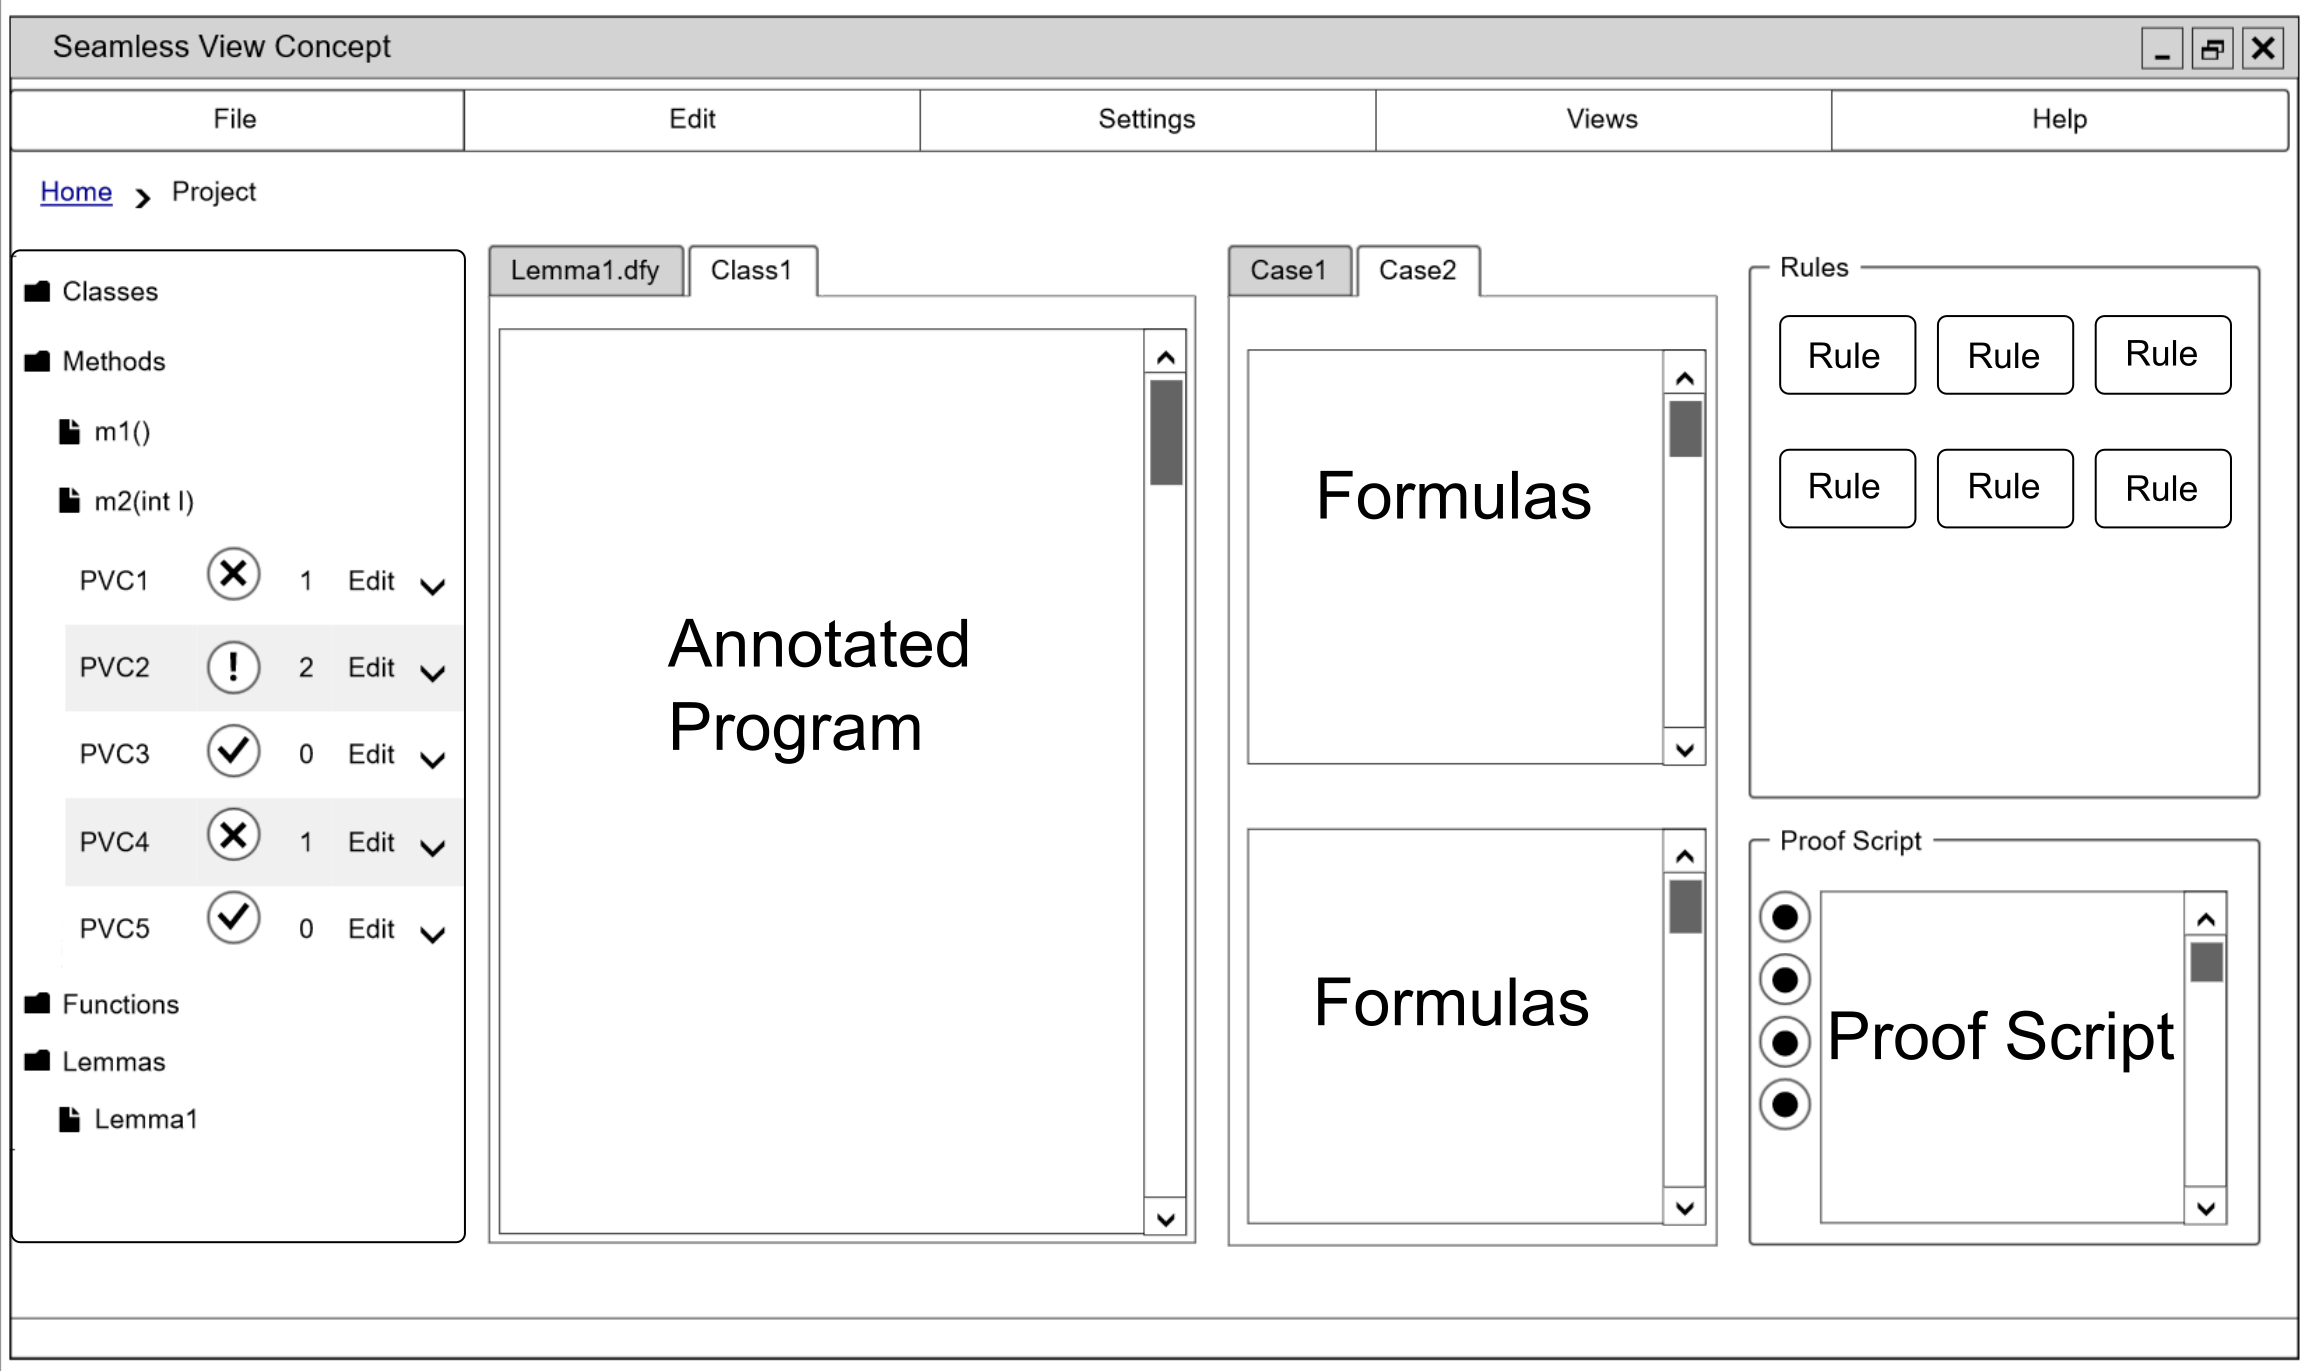
\includegraphics[width=\textwidth]{imagesEnglish/abstractConceptViews.png}};
 \draw[color=white] (-6.1,3.6) rectangle (5.9,-3.4);
% % \node[circle=2pt,fill=black] (foo) at (0,-2) {};
 \only<2>{\draw[color=KITgreen, line width=1.5mm] (-6,3.5) rectangle (0.5,-3.4);}
 \only<3>{\draw[color=KITgreen, line width=1.5mm] (-3.4,3.5) rectangle (3,-3.4);}
 \only<4>{\draw[color=KITgreen, line width=1.5mm] (0,3.5) rectangle (5.9,-3.4);}
 
% \draw[](1,0) -- (0,0);
\end{tikzpicture} 
\end{center}

\end{frame}

\begin{frame}{Exemplary Walkthrough}

\begin{tikzpicture}[
spy using outlines={
  rectangle,
  magnification=2,
  connect spies}]
\node[inner sep=0pt] {\pgfimage[width=\textwidth]{imagesEnglish/screenshots/view-21.png}};
\only<2>{\spy[KITgreen,width=5cm, height=.5cm] on (-4.1,0.15) in node at (.1\textwidth,2);
\spy[KITgreen, width=3.5cm, height=.5cm] on (1.35,-1.25) in node at (.1\textwidth,-2.5);}
\end{tikzpicture}
\end{frame}

\begin{frame}{Exemplary Walkthrough}
%9
\begin{tikzpicture}[]
\node (img1)  { 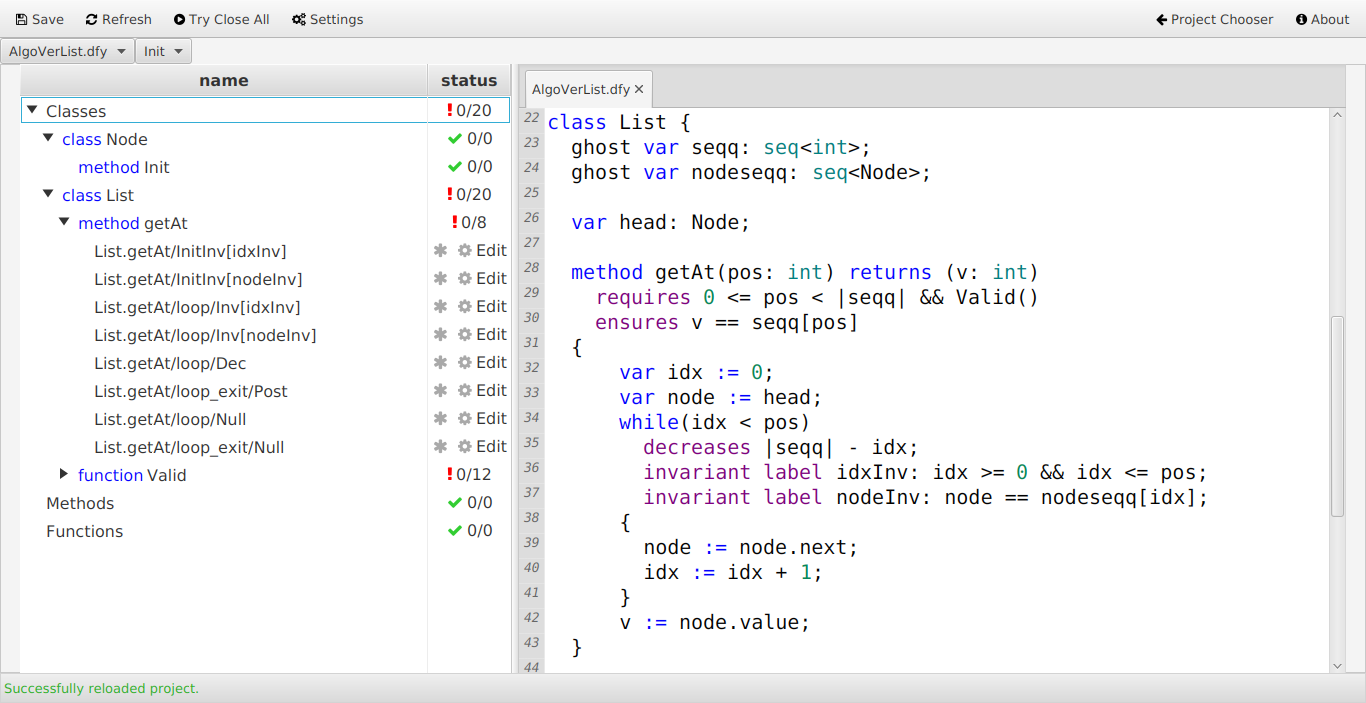
\includegraphics[width=\textwidth]{imagesEnglish/screenshots/view-21.png}};
 \draw[color=white] (-6.1,3.6) rectangle (5.9,-3.7);
% % \node[circle=2pt,fill=black] (foo) at (0,-2) {};
  \only<2>{\node (img1)  { 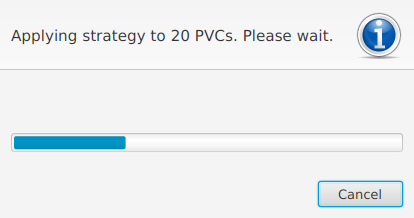
\includegraphics[width=.5\textwidth,frame]{imagesEnglish/screenshots/view-1.png}};}
  \only<3>{\node (img1)  { 
\includegraphics[width=.5\textwidth,frame]{imagesEnglish/screenshots/view-2.png}};}
%  \only<3>{\draw[color=KITgreen, line width=1.5mm] (-3.4,3.5) rectangle (3,-3.7);}
%  \only<4>{\draw[color=KITgreen, line width=1.5mm] (0,3.5) rectangle (5.9,-3.6);}
\end{tikzpicture} 

\end{frame}

\begin{frame}{Exemplary Walkthrough}
 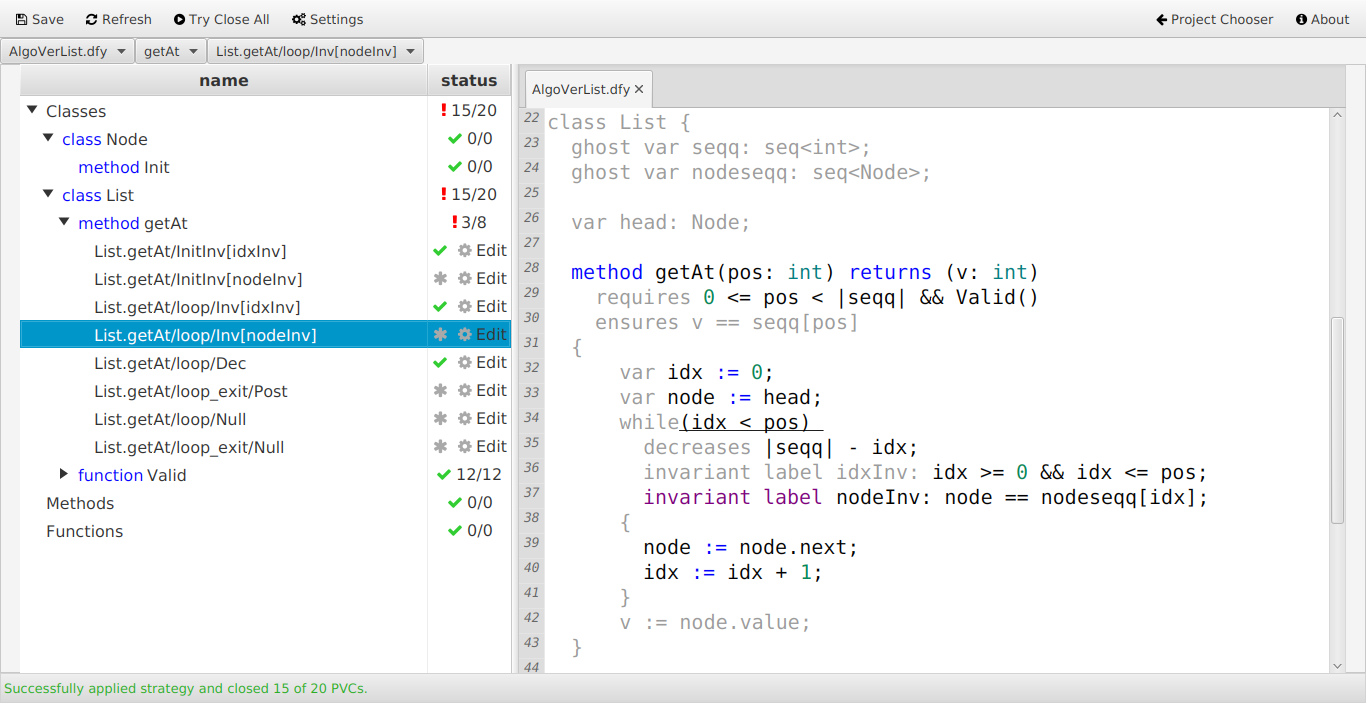
\includegraphics[width=\textwidth]{imagesEnglish/screenshots/view-22.png}

\end{frame}
\begin{frame}{Exemplary Walkthrough}
 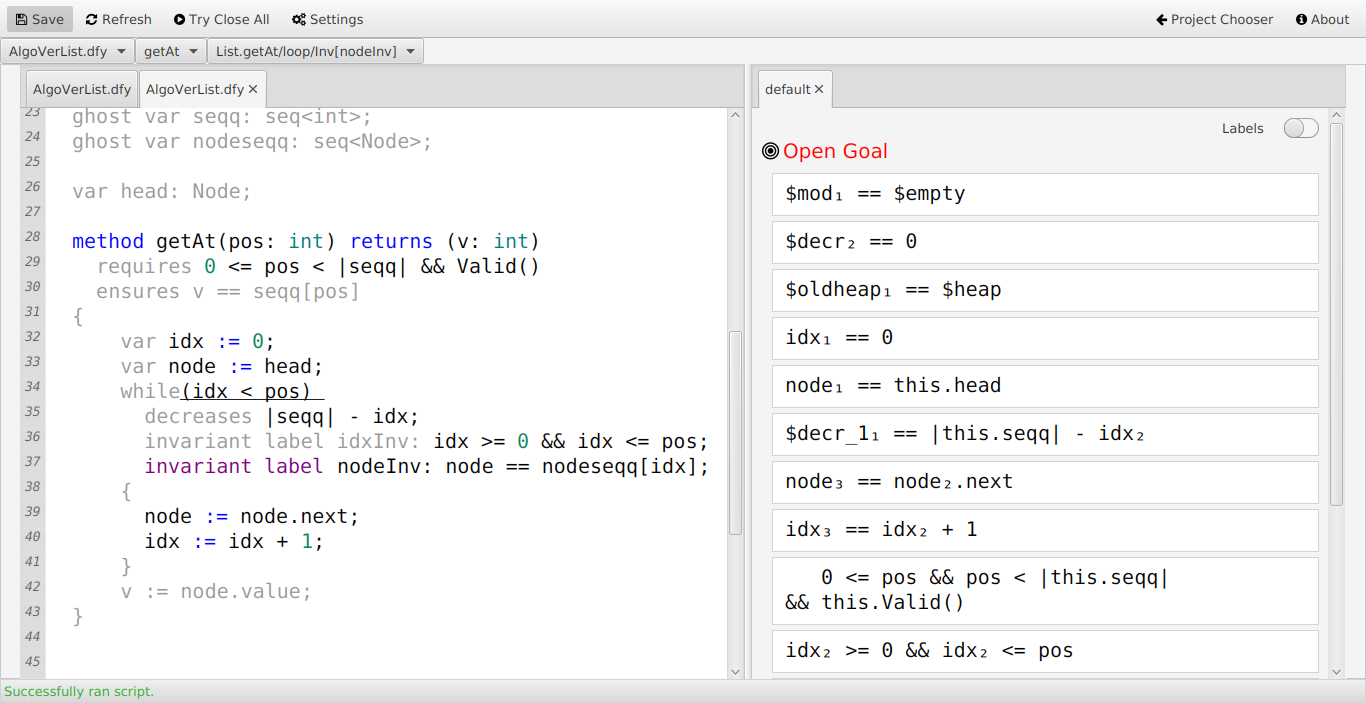
\includegraphics[width=\textwidth]{imagesEnglish/screenshots/view-24.png}

\end{frame}
\begin{frame}{Exemplary Walkthrough}
 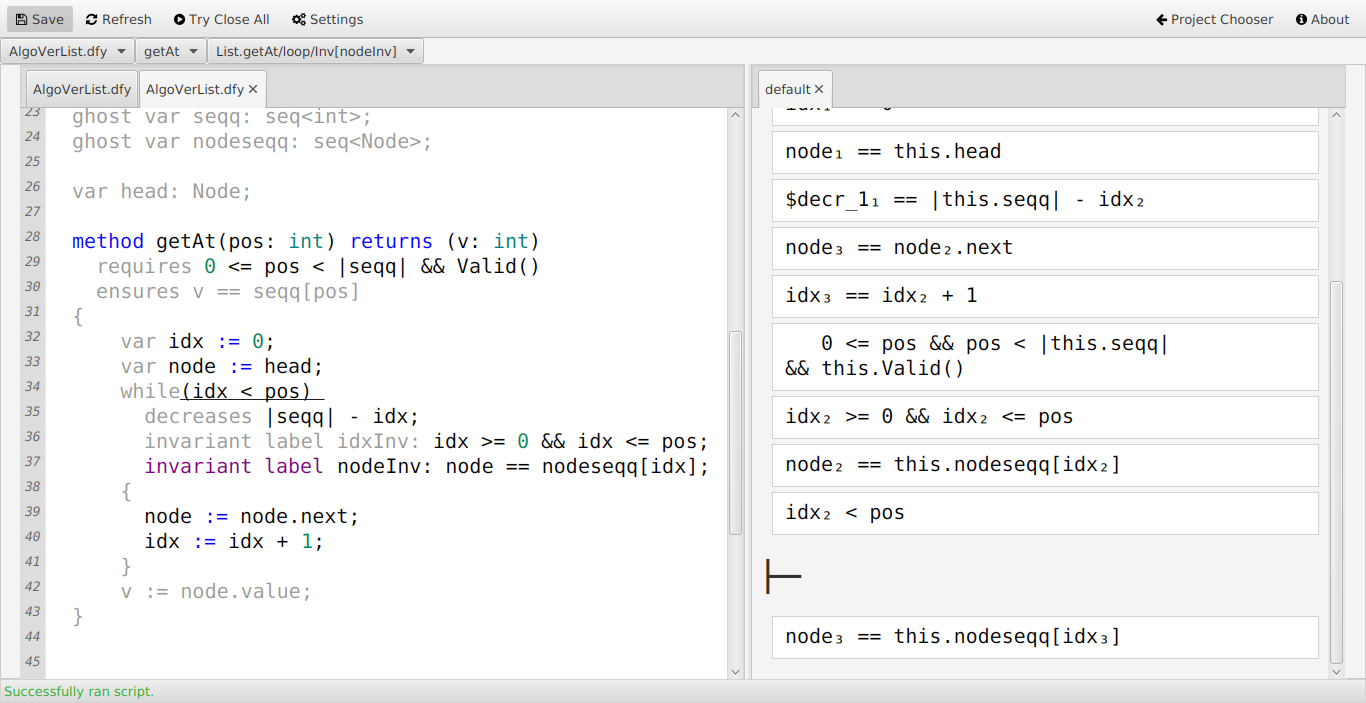
\includegraphics[width=\textwidth]{imagesEnglish/screenshots/view-23.png}

\end{frame}
\begin{frame}{Exemplary Walkthrough}
 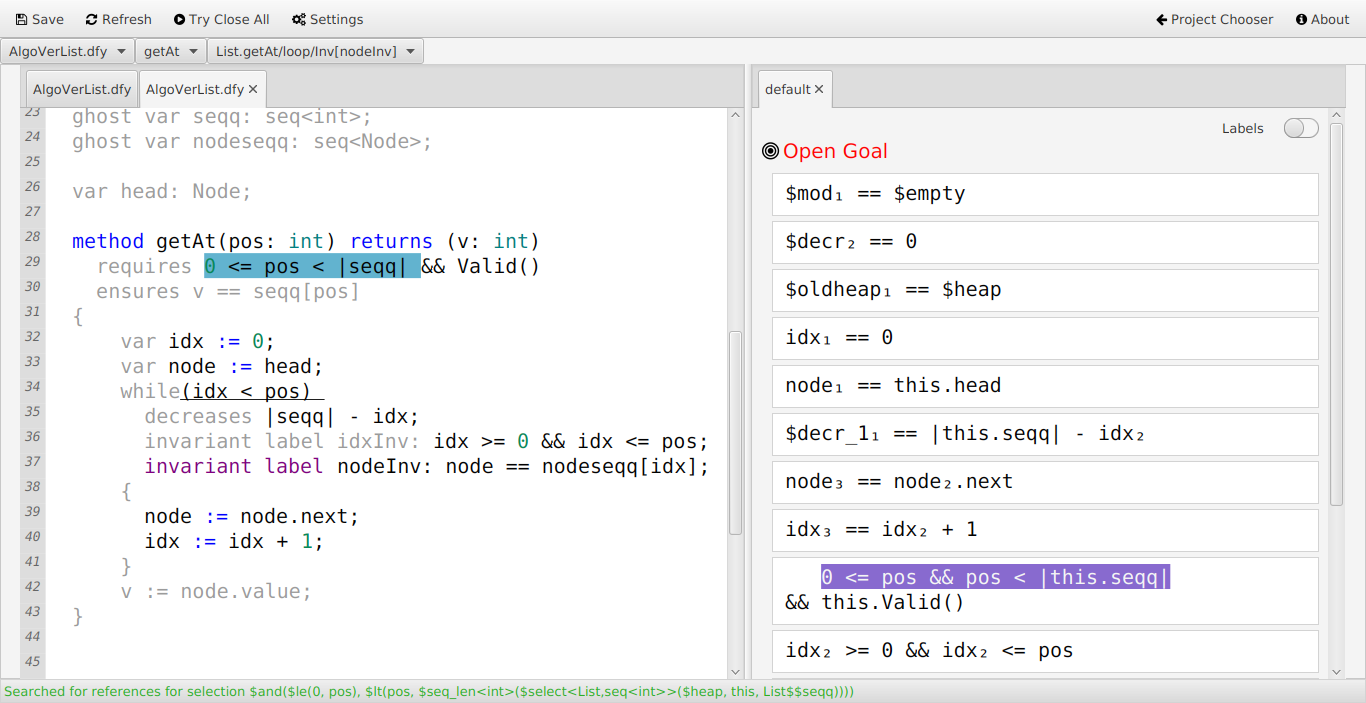
\includegraphics[width=\textwidth]{imagesEnglish/screenshots/view-25.png}

\end{frame}
\begin{frame}{Exemplary Walkthrough}
 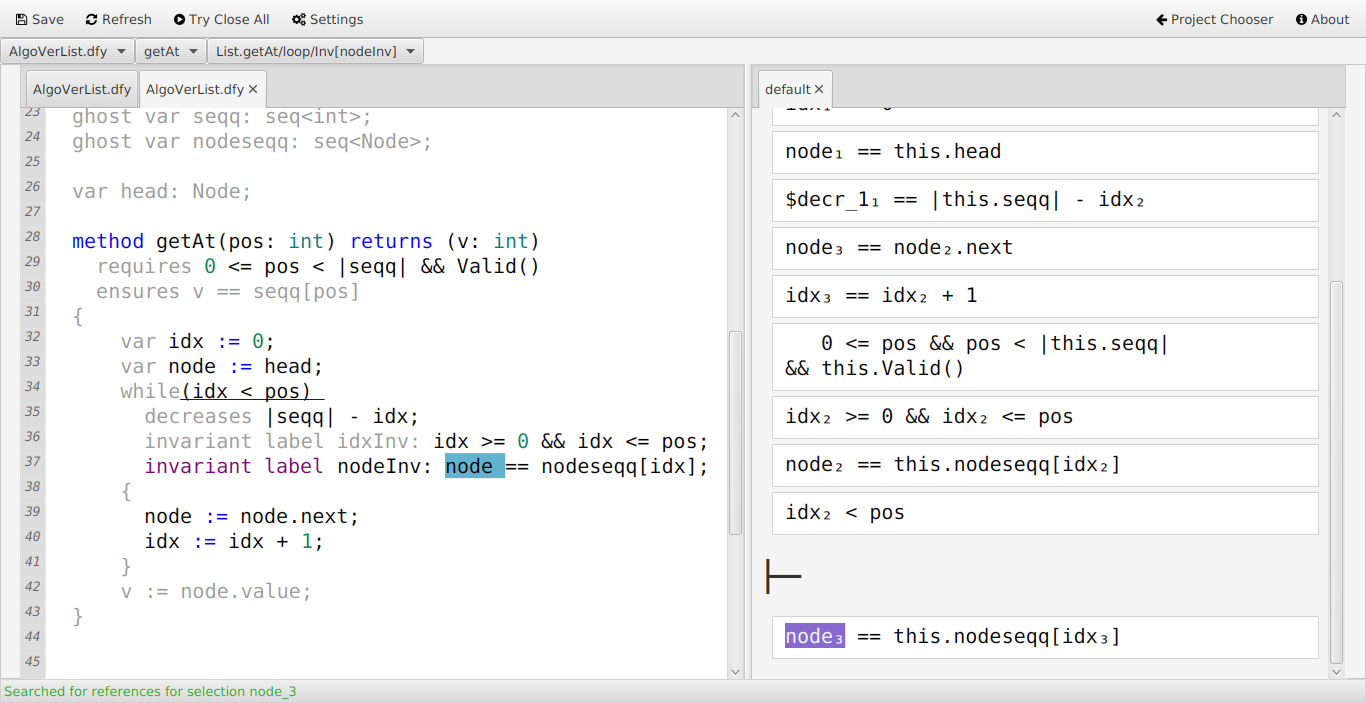
\includegraphics[width=\textwidth]{imagesEnglish/screenshots/view-26.png}

\end{frame}
\begin{frame}{Exemplary Walkthrough}
 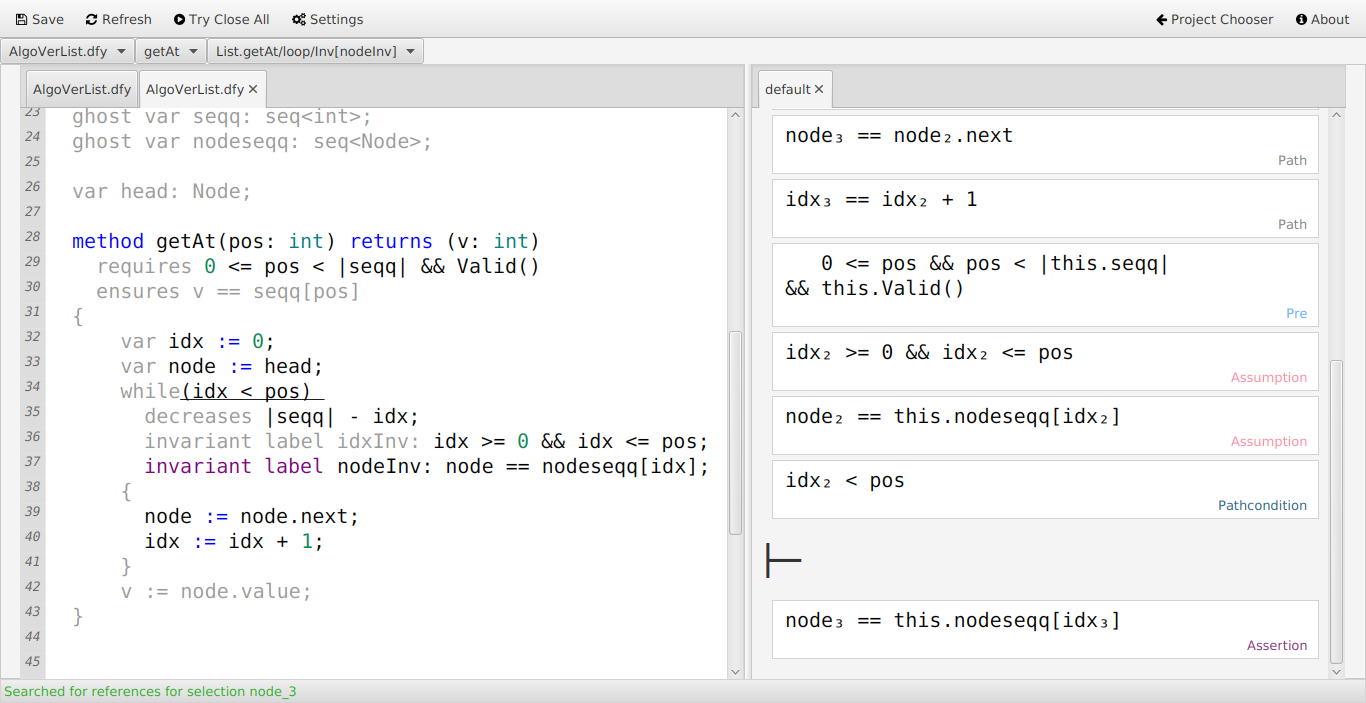
\includegraphics[width=\textwidth]{imagesEnglish/screenshots/view-27.png}

\end{frame}
\begin{frame}{Exemplary Walkthrough}
%  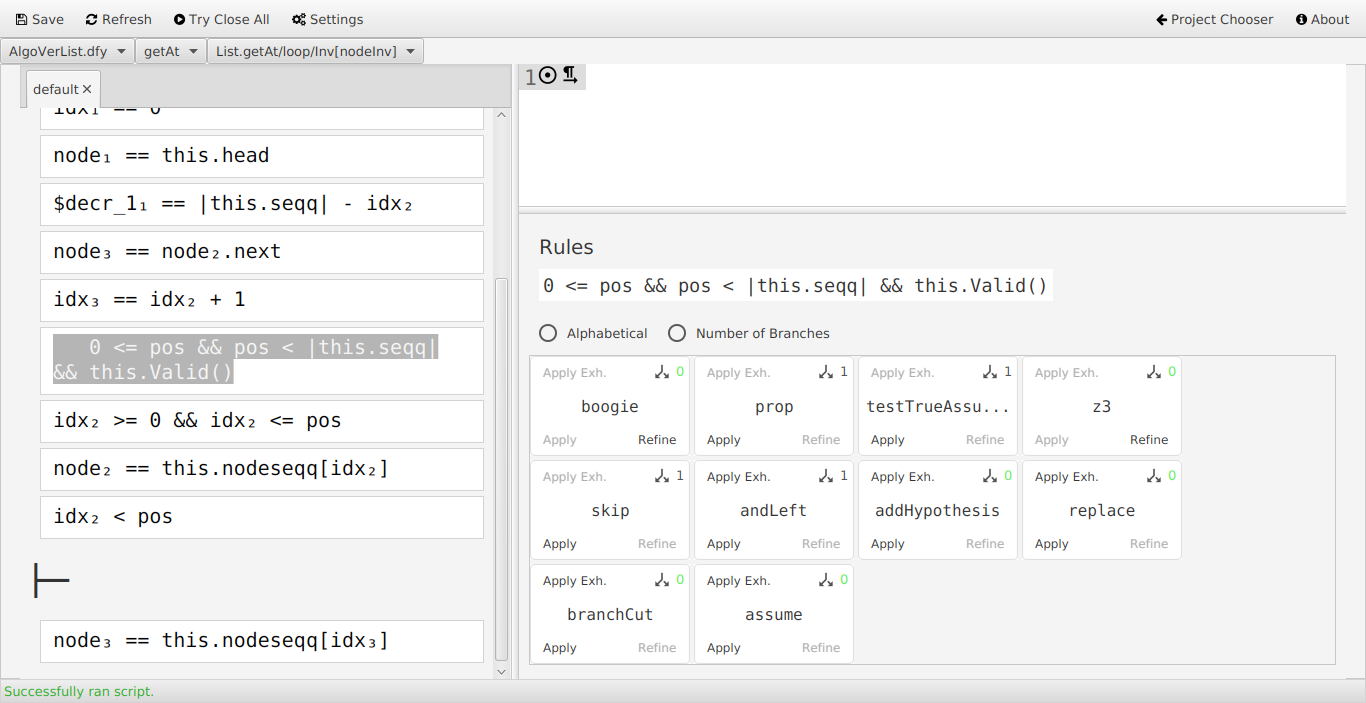
\includegraphics[width=\textwidth]{imagesEnglish/screenshots/view-28.png}
%  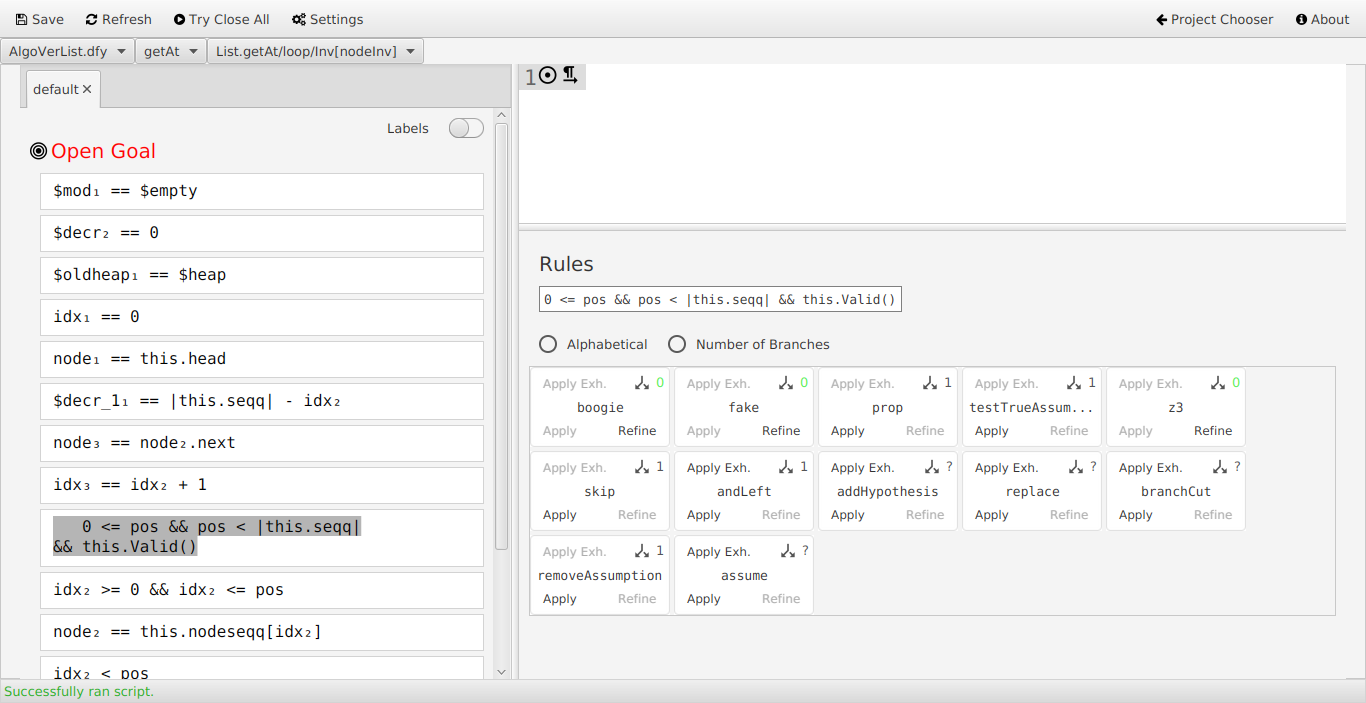
\includegraphics[width=\textwidth]{imagesEnglish/screenshots/viewNew.png}

\begin{tikzpicture}[
spy using outlines={
  rectangle,
  magnification=2,
  connect spies}]
\node[inner sep=0pt] {\pgfimage[width=\textwidth]{imagesEnglish/screenshots/viewNew.png}};
\only<2>{\spy[KITgreen,width=3cm, height=2cm] on (0.5,-1.3) in node at (.1\textwidth,2);
}
\end{tikzpicture}
\end{frame}

\begin{frame}{Exemplary Walkthrough}
 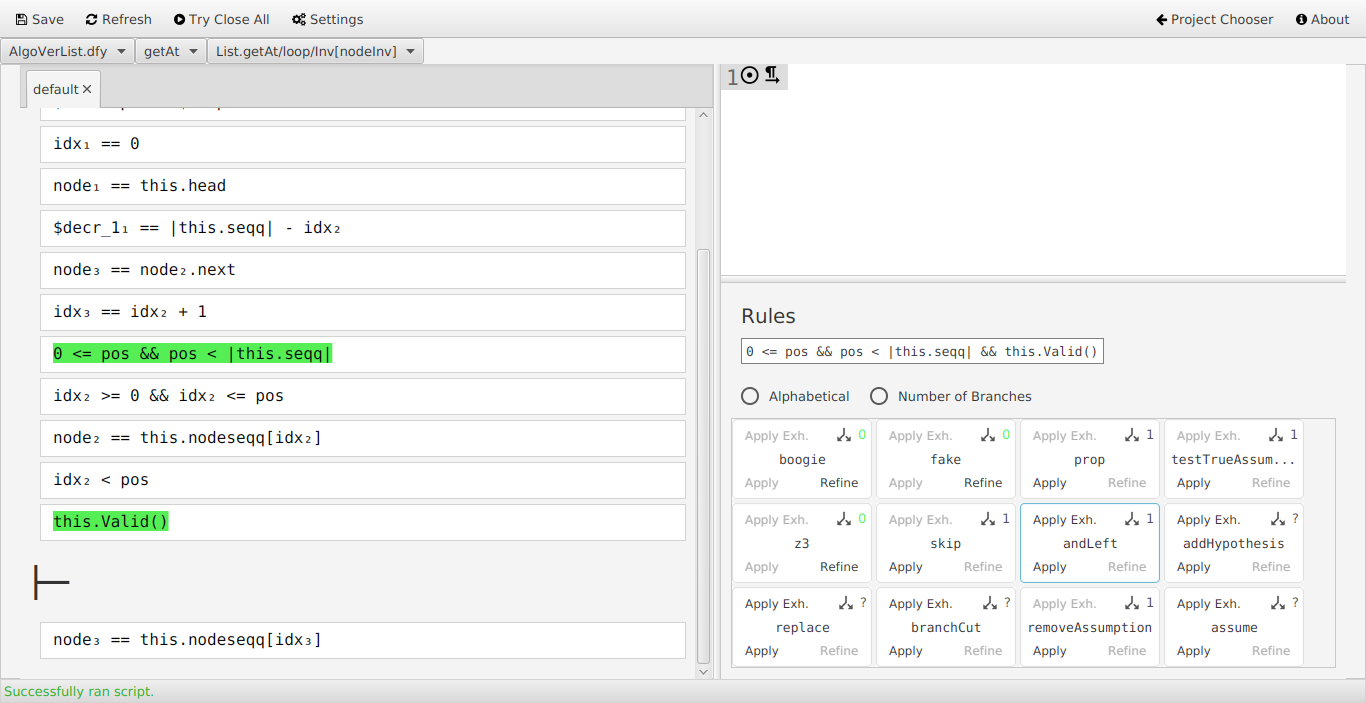
\includegraphics[width=\textwidth]{imagesEnglish/screenshots/viewNew-6.png}
%view-29.png
\end{frame}


\begin{frame}{Exemplary Walkthrough}
 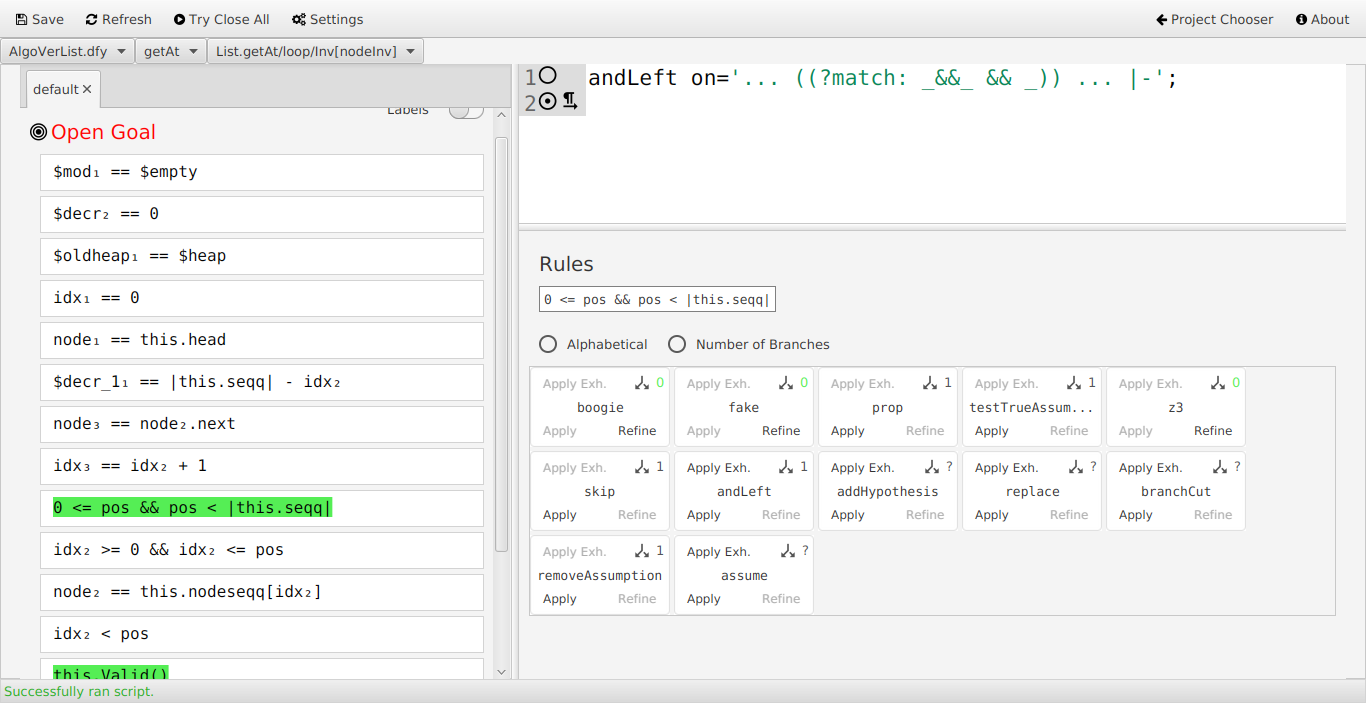
\includegraphics[width=\textwidth]{imagesEnglish/screenshots/viewNew-1.png}
%view-29.png
\end{frame}

\begin{frame}{Exemplary Walkthrough}
 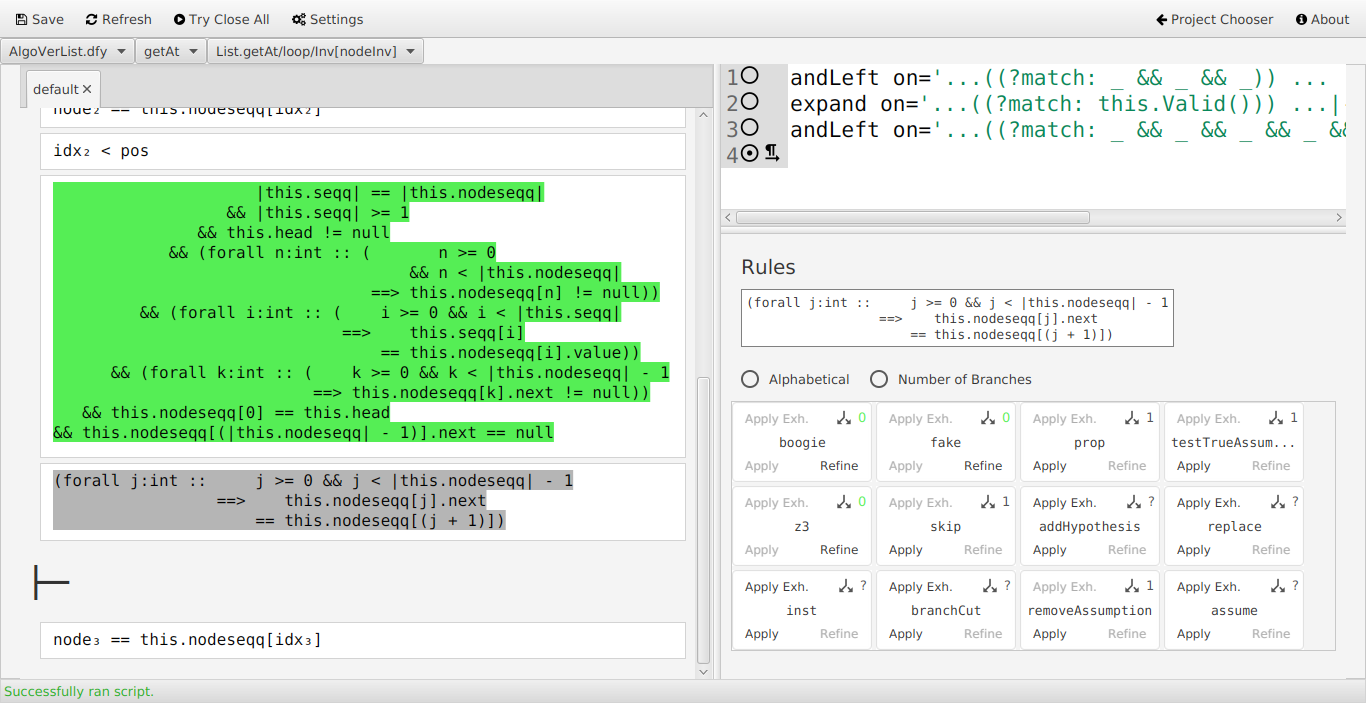
\includegraphics[width=\textwidth]{imagesEnglish/screenshots/viewNew-2.png}
%view-30.png
\end{frame}

\begin{frame}{Exemplary Walkthrough}
%  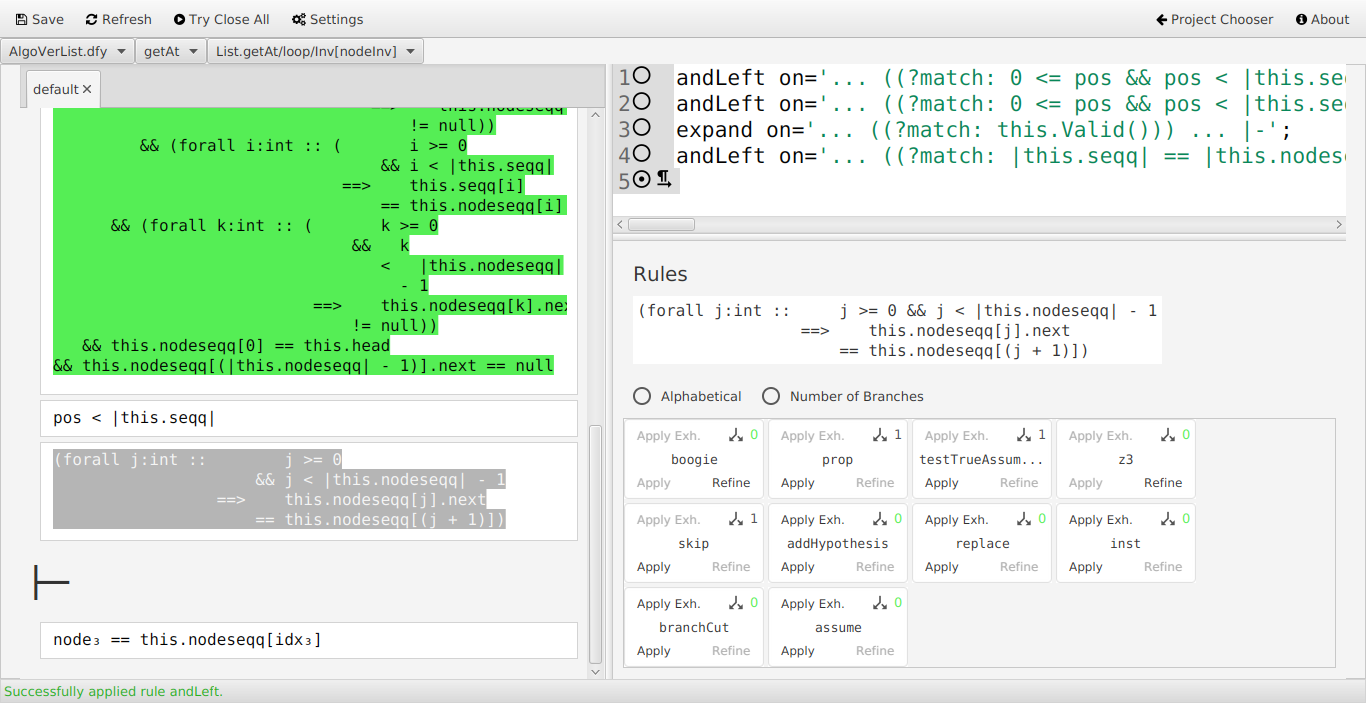
\includegraphics[width=\textwidth]{imagesEnglish/screenshots/view-31.png}
\begin{tikzpicture}[]
\node (img1)  { 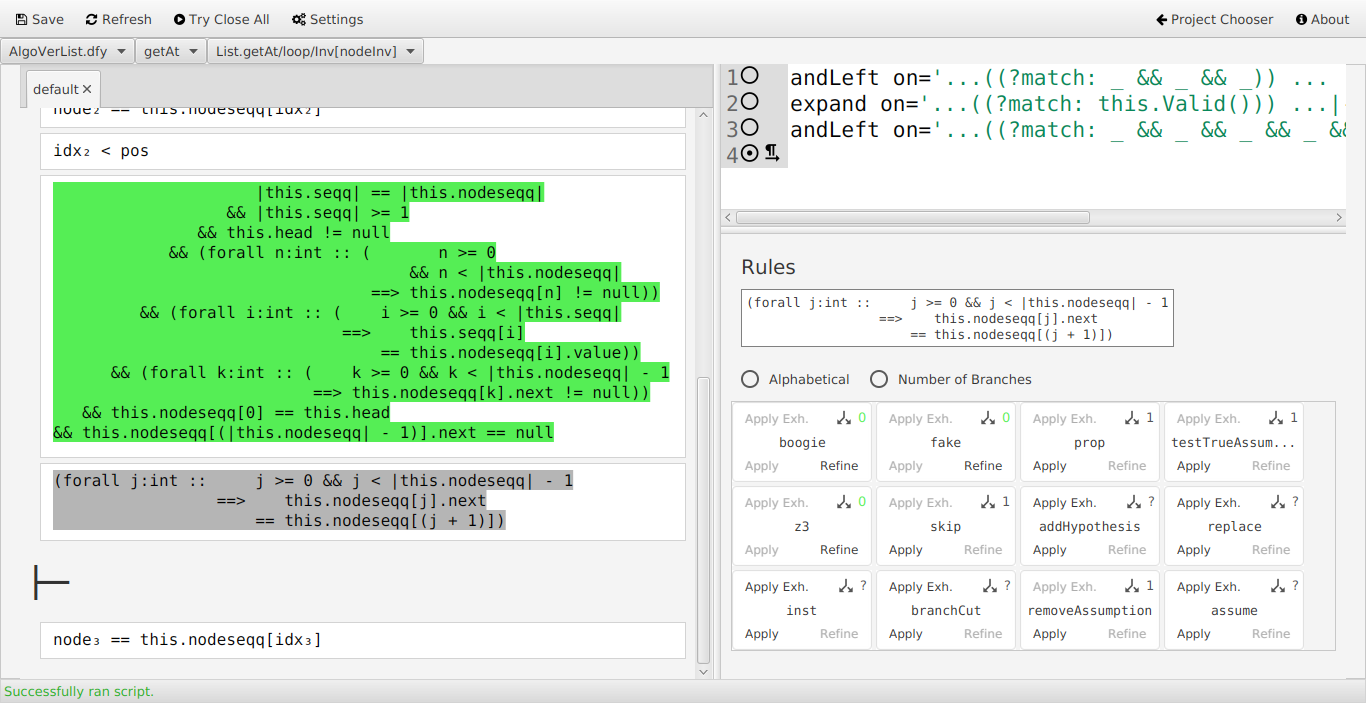
\includegraphics[width=\textwidth]{imagesEnglish/screenshots/viewNew-2.png}};
 \draw[color=white] (-6.1,3.6) rectangle (5.9,-3.7);
% % \node[circle=2pt,fill=black] (foo) at (0,-2) {};
  \only<2>{\node (img1)  { 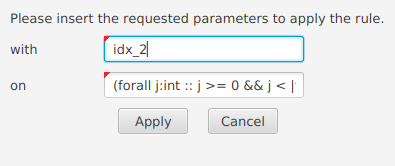
\includegraphics[width=.4\textwidth,frame]{imagesEnglish/screenshots/view-16.png}};}
%  \only<3>{\draw[color=KITgreen, line width=1.5mm] (-3.4,3.5) rectangle (3,-3.7);}
%  \only<4>{\draw[color=KITgreen, line width=1.5mm] (0,3.5) rectangle (5.9,-3.6);}
\end{tikzpicture} 

\end{frame}

\begin{frame}{Exemplary Walkthrough}
 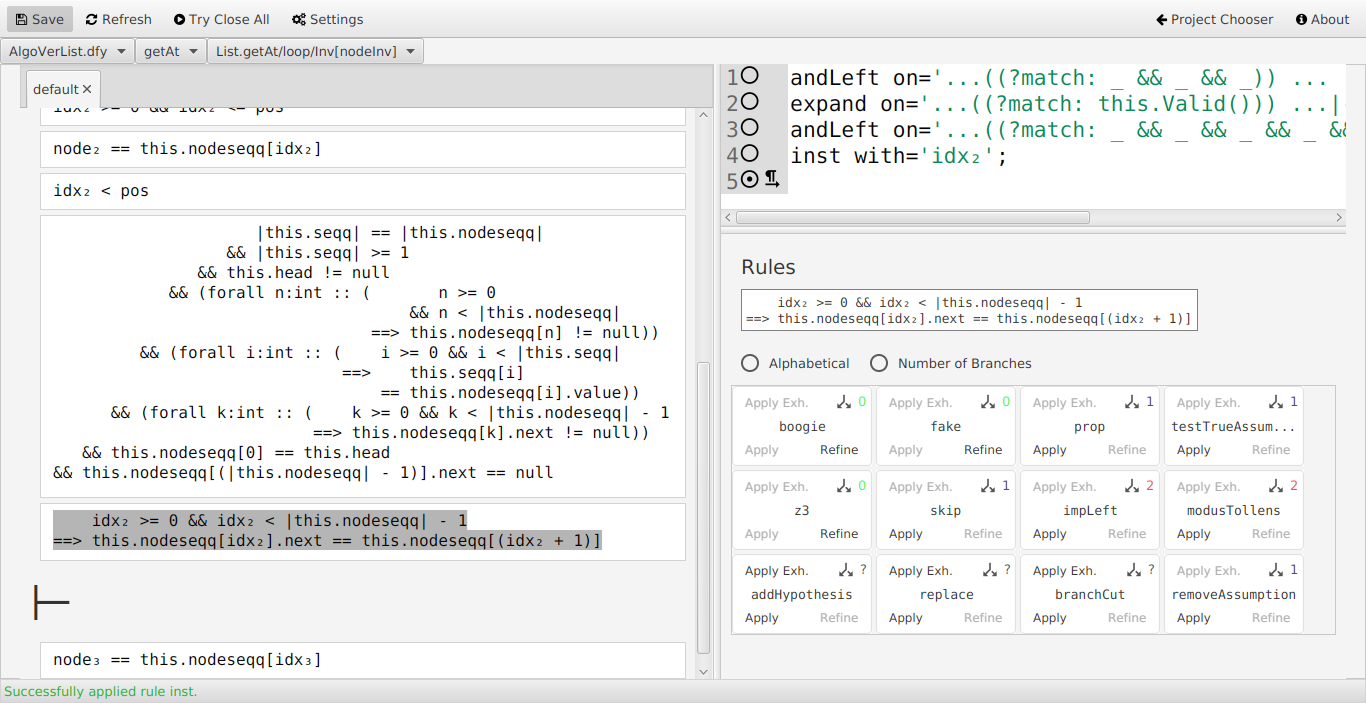
\includegraphics[width=\textwidth]{imagesEnglish/screenshots/viewNew-3.png}
% view-32.png
\end{frame}

\begin{frame}{Exemplary Walkthrough}
 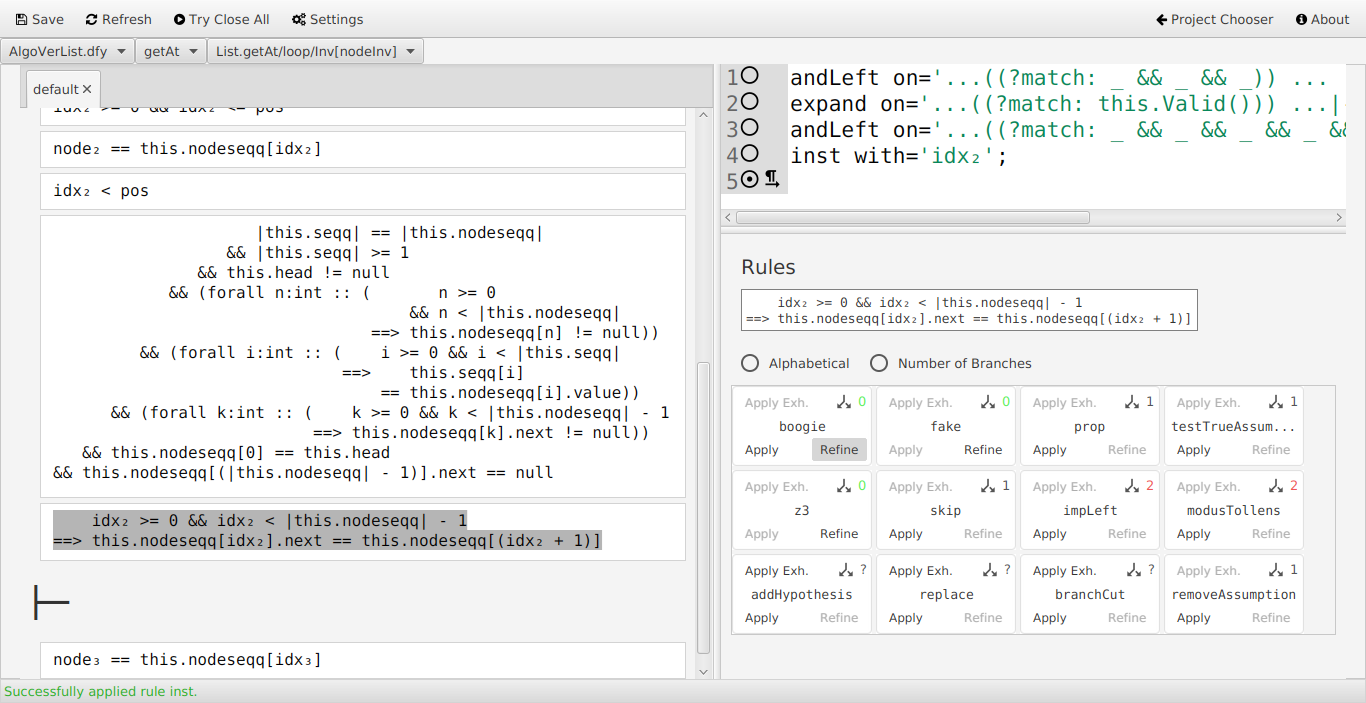
\includegraphics[width=\textwidth]{imagesEnglish/screenshots/viewNew-4.png}
% view-32.png
\end{frame}

\begin{frame}{Exemplary Walkthrough}
 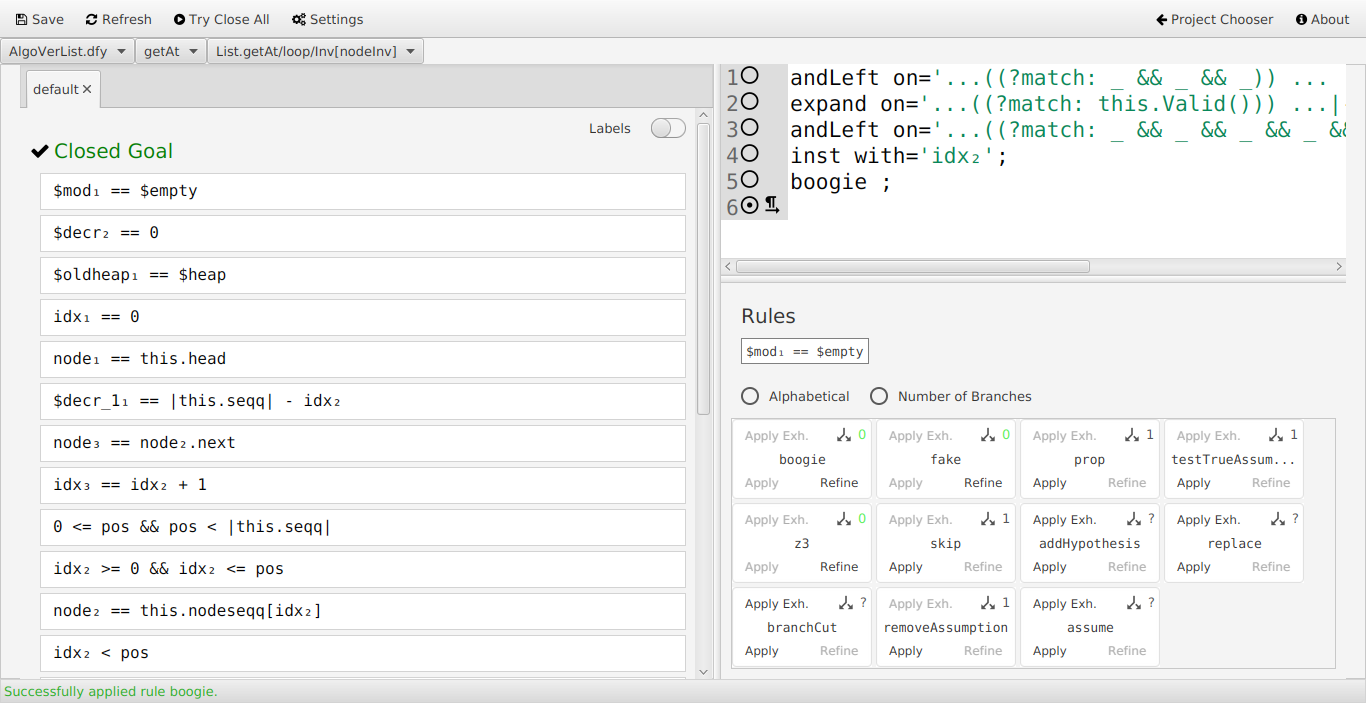
\includegraphics[width=\textwidth]{imagesEnglish/screenshots/viewNew-5.png}
% view-32.png
\end{frame}

\begin{frame}{Relation in the Proof}
 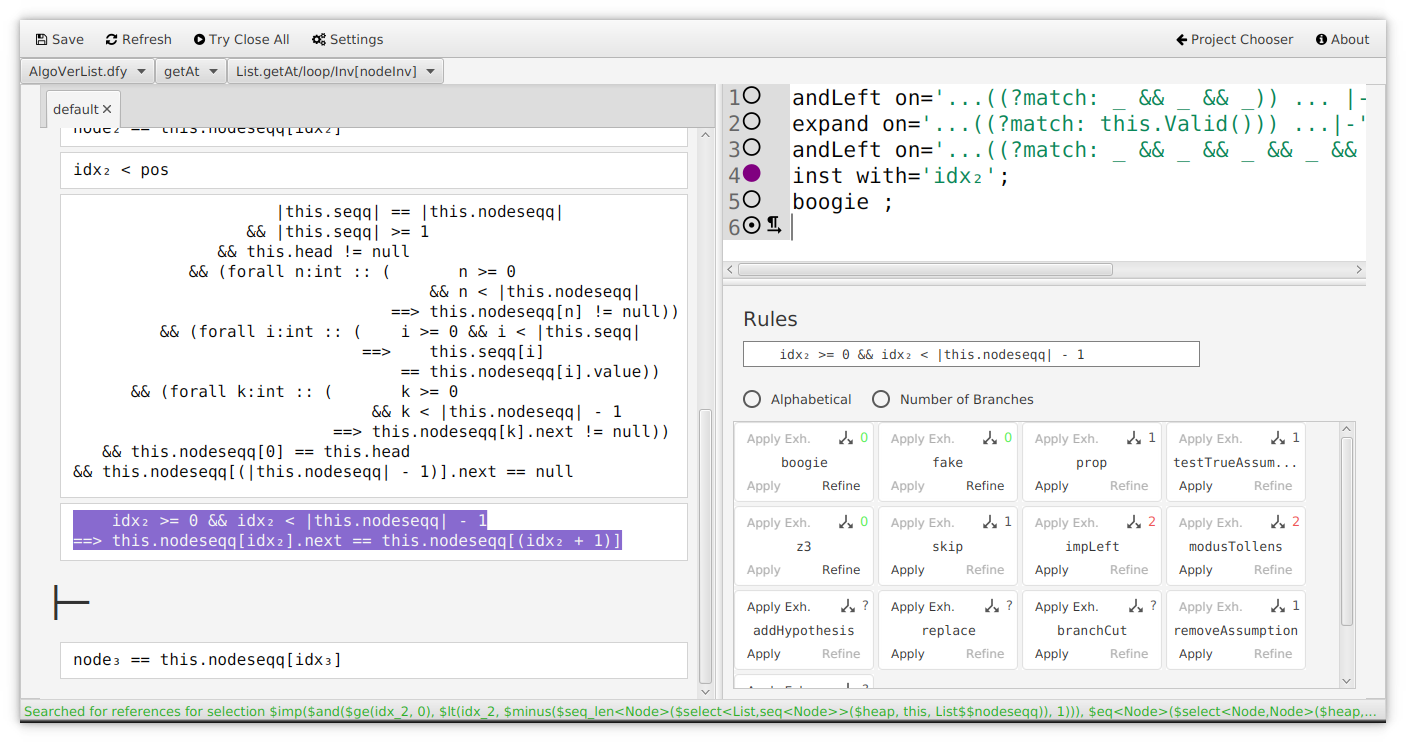
\includegraphics[width=\textwidth]{imagesEnglish/screenshots/viewNew-9.png}
% view-32.png
\end{frame}

\begin{frame}{Relation in the Proof}
 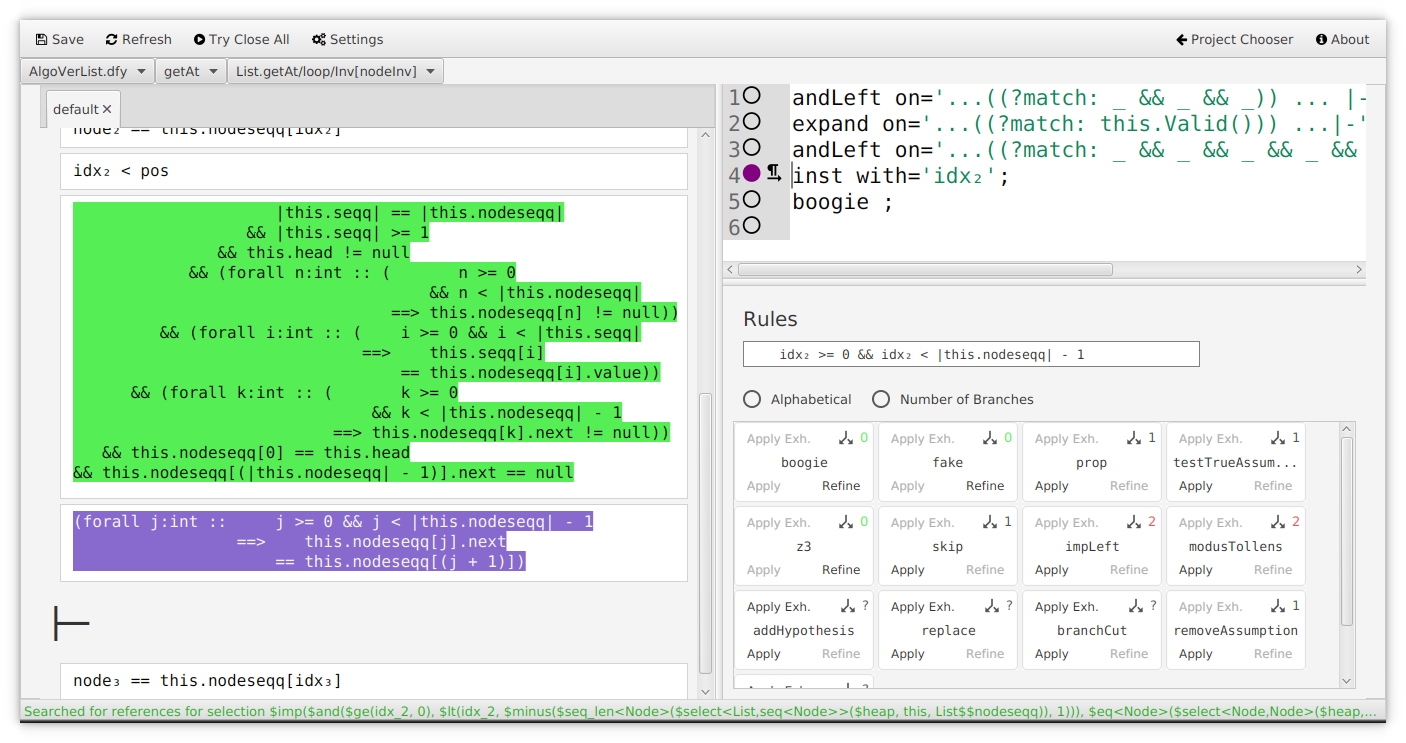
\includegraphics[width=\textwidth]{imagesEnglish/screenshots/viewNew-10.png}
% view-32.png
\end{frame}

\begin{frame}{Relation in the Proof}
 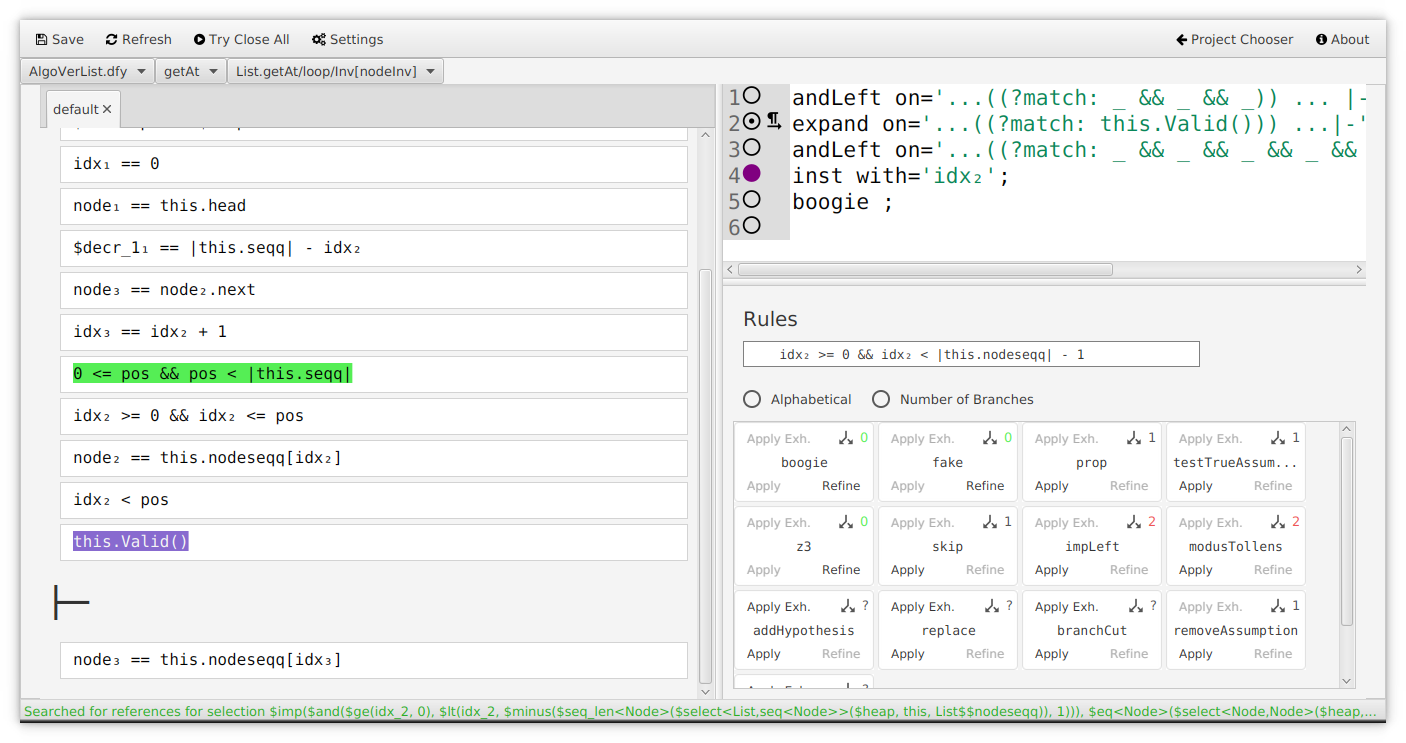
\includegraphics[width=\textwidth]{imagesEnglish/screenshots/viewNew-11.png}
% view-32.png
\end{frame}


\begin{frame}{Branching in a Proof}
 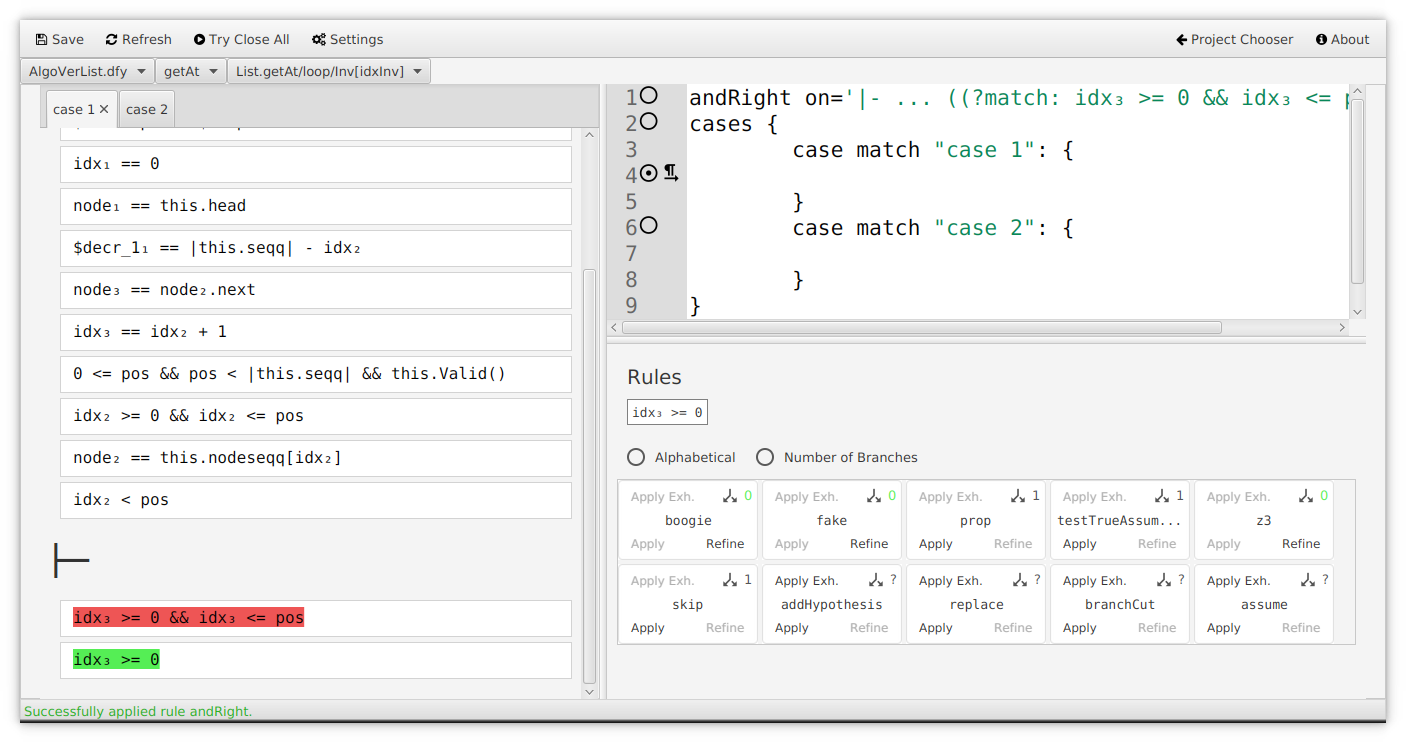
\includegraphics[width=\textwidth]{imagesEnglish/screenshots/viewNew-8.png}

\end{frame}


\begin{frame}{Further Features and WIP}
\begin{itemize}
 \item simple lemmas can be encoded using Dafny syntax allowing to add rewrite rules
 \item call and callsite information is available
\end{itemize}

 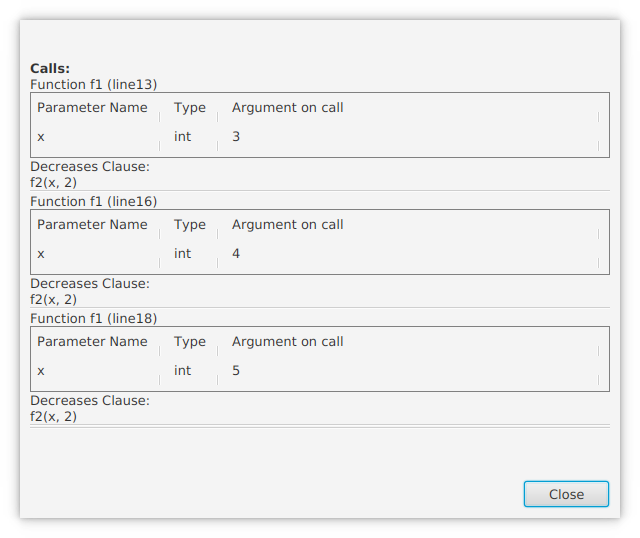
\includegraphics[width=.6\textwidth]{imagesEnglish/screenshots/viewNew-7.png}
% view-32.png
\end{frame}



\begin{frame}{Related Work}
 \begin{block}{Provide different views}
  e.g., KIV, Why3, \KeY{}, \KeY{}maeraX, Coq, Isabelle,...
\end{block}

\begin{block}{Combination of automation and interaction}
 Why3 (hierachical structuring of proof task and usage of different solvers)
\end{block}
%%meist hoert nach zwei View auf
\begin{block}{Interaction styles}
\begin{itemize}
\item auto-active verification:  VCC, Dafny, OpenJML
\item direct manipulation: \KeY{}, \KeY{}maeraX, KIV
\item text-based: Coq, Isabelle
\item combination direct manipulation + text-based: \KeY{}maeraX
\end{itemize}
\end{block}
\begin{block}{Verification IDEs}
 e.g., Why3, DafnyIDE 
\end{block}

\end{frame}



\begin{frame}{Summary and Conclusion}
\begin{block}{Our Contributions}
 \begin{itemize}
  \item qualitative user studies on interaction in interactive verification systems
  \item a new user interaction concept 
  \begin{itemize}
  \item combination of different interaction styles 
  \item application of usability principles\\ (e.g., visual clarity, substituitivity, anticipation, consistency, ...)
  \item integration of supporting features
  \end{itemize}
  
  \item an implementation of the concept in the research prototype DIVE
  (\Large{\url{https://github.com/mattulbrich/dive}})
 \end{itemize}

\end{block}
\end{frame}
\begin{frame}[t]{Summary and Conclusion}
\begin{block}{Conclusion}
 \begin{itemize}
  \item proof state comprehension is one of the central issues
  \item there is not one single interaction strategy
  \item interaction styles can be combined for an improved user support
 \end{itemize}

\end{block}


\begin{block}{Future Work}
\begin{itemize}
 \item encode user interactions back to annotations
 \item include counter examples in the DIVE user interface
 \item larger case studies and quantitative user studies
\end{itemize}
\end{block}
\end{frame}

\begin{frame}
\begin{center}

 \Large{Thank you for your attention!}\\
 \bigskip
\huge{\url{https://github.com/mattulbrich/dive}}
 
\includegraphics[width=.4\textwidth]{imagesEnglish/logo.png}
\end{center}

\end{frame}

\begin{frame}{Consolidated Sequence Model}
\begin{center}
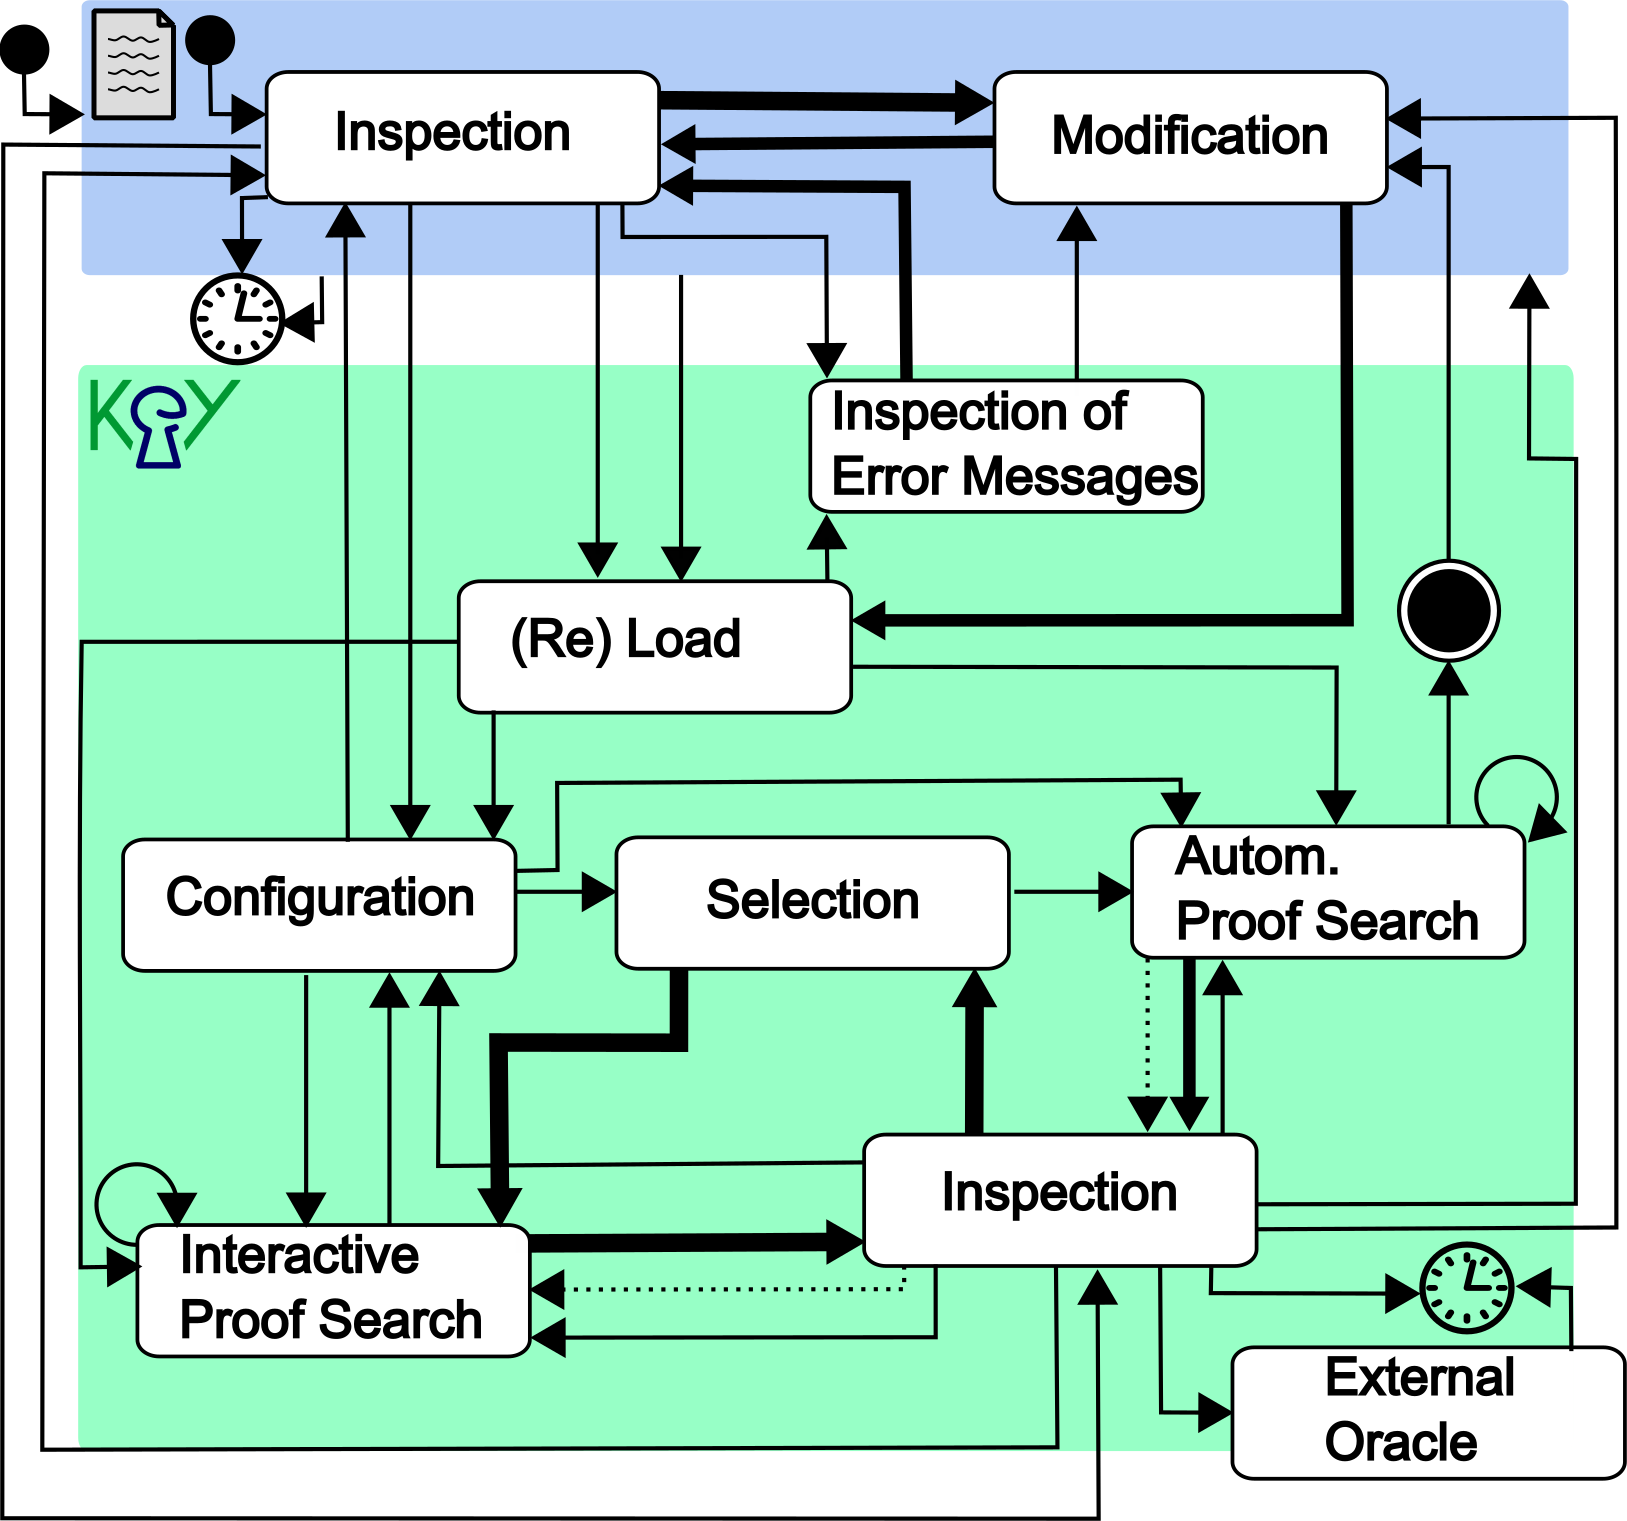
\includegraphics[height=\textheight]{imagesEnglish/consolidatedProcessNewLine.png} 
 
\end{center}

\end{frame}

\begin{frame}{Model of Process}
\begin{center}
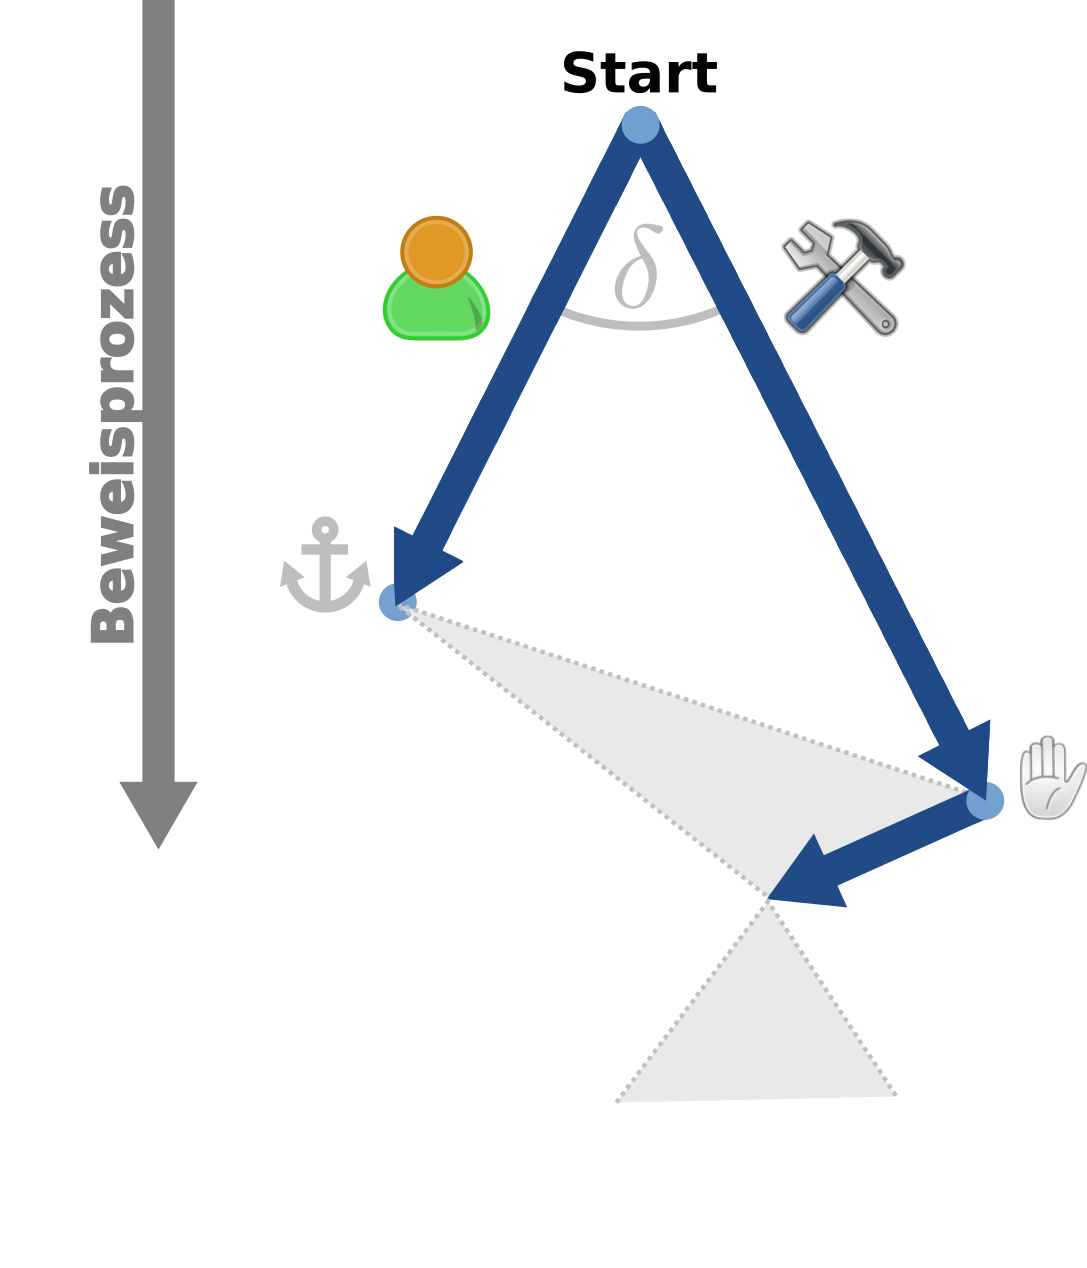
\includegraphics[height=\textheight]{imagesEnglish/gap.png} 
 
\end{center}

\end{frame}

\begin{frame}{Model of Process}
\begin{center}
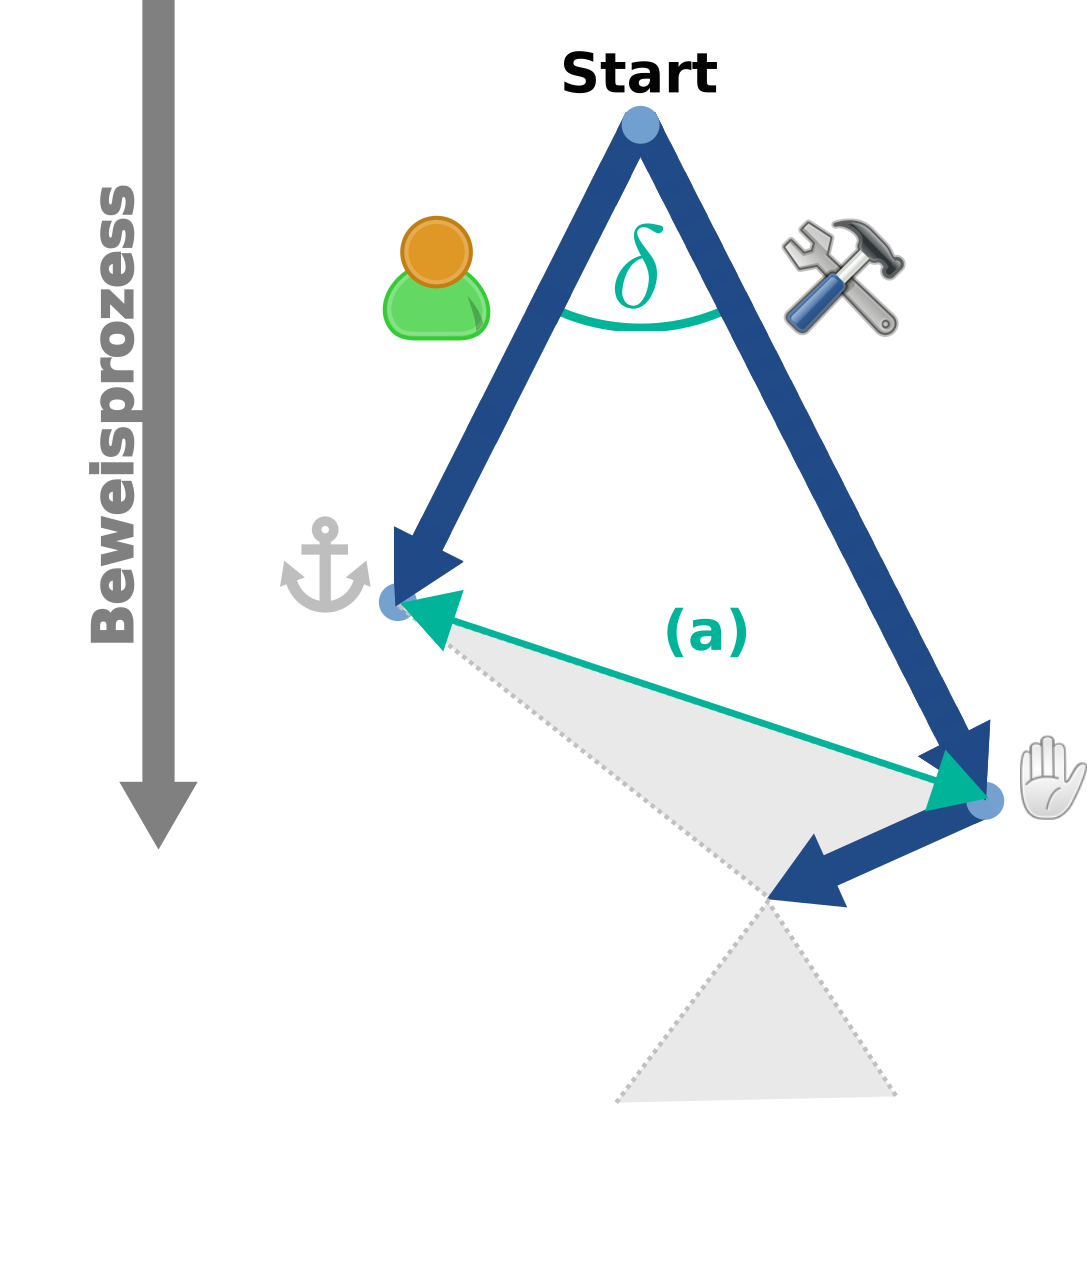
\includegraphics[height=\textheight]{imagesEnglish/gapA.png} 
 
\end{center}

\end{frame}
\begin{frame}{Model of Process}
\begin{center}
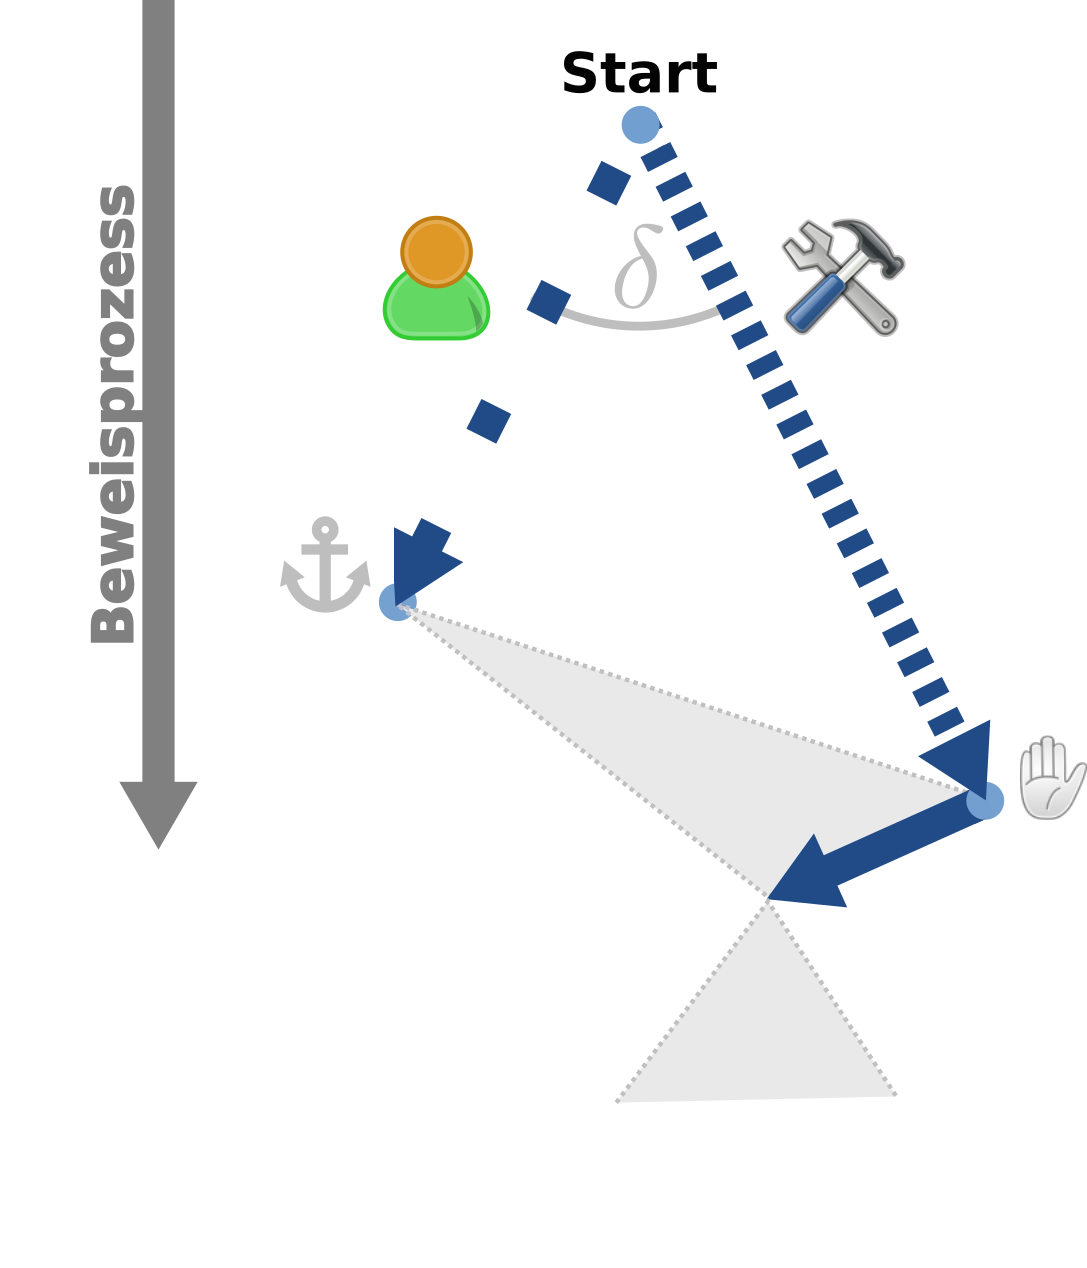
\includegraphics[height=\textheight]{imagesEnglish/gapB.png} 
 
\end{center}

\end{frame}
\begin{frame}{Model of Process}
\begin{center}
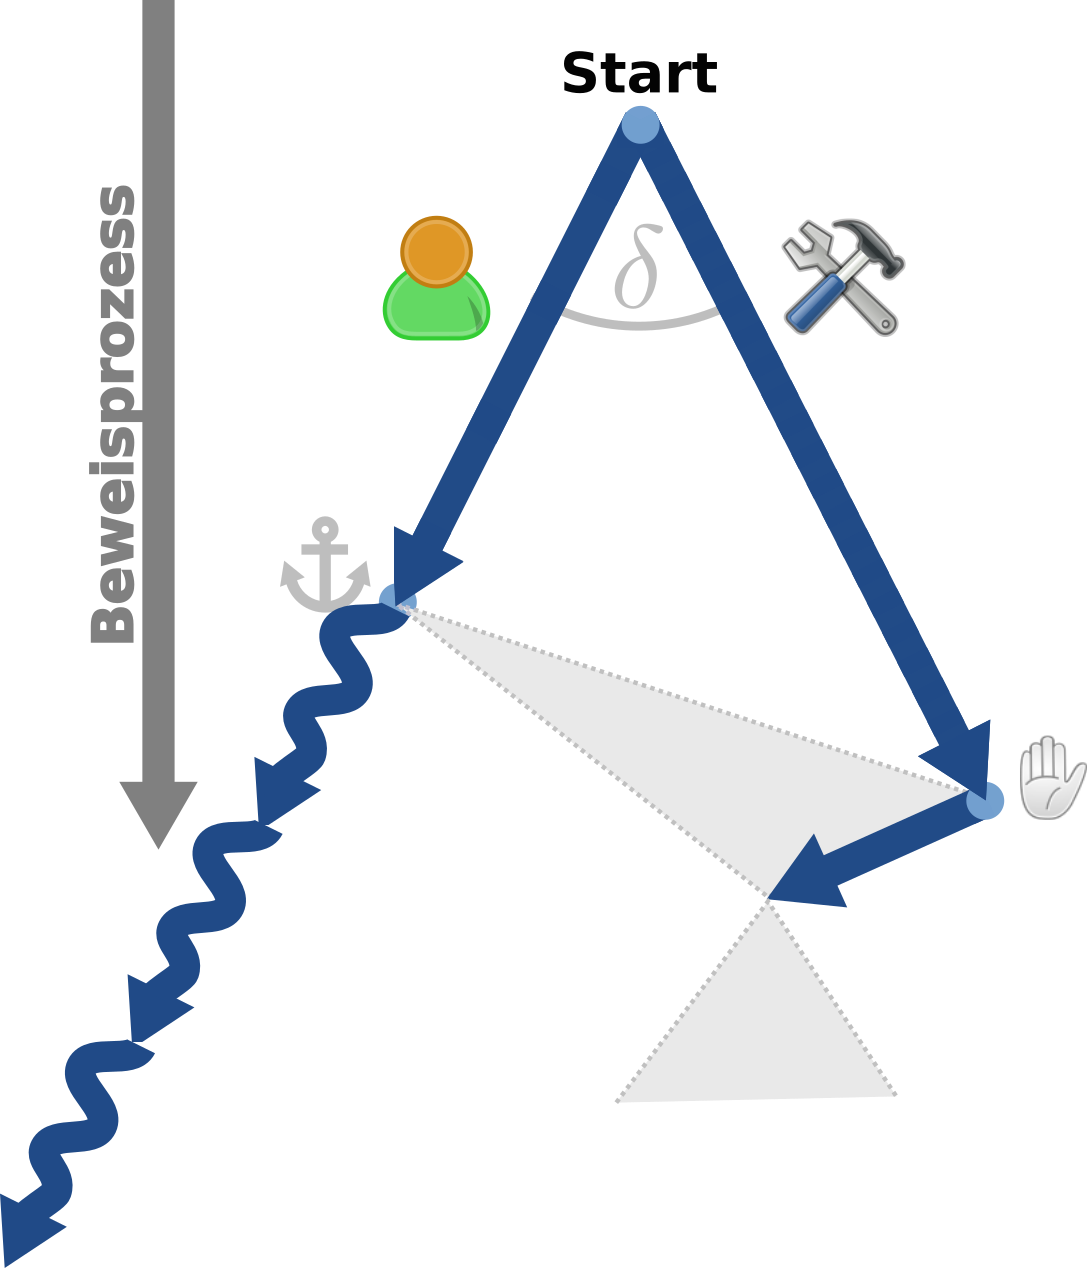
\includegraphics[height=\textheight]{imagesEnglish/gapC.png} 
 
\end{center}

\end{frame}

\end{document}

